%-------------------------------------------------------%
%       Snakemake-Intro for HPC Users                   %
%-------------------------------------------------------%

\documentclass[english,xcolor=pdftex,dvipsnames]{beamer} 

% to typeset only a few slide sets, set them here during development
%\includeonly{Why_Workflows}

\usepackage{etoolbox}
%\setbeamertemplate{mini frames}[box]
\usepackage{babel}
\usepackage[utf8]{inputenc}
\usepackage[T1]{fontenc}
\usepackage{amsfonts,amsmath,amssymb}
\usepackage{textgreek}
\usepackage{wrapfig}

\usepackage[load-configurations=binary,binary-units=true]{siunitx}
\usepackage[normalem]{ulem} % for strikethrough with \sout

\usepackage{color,colortbl}
\usepackage{upquote}

\definecolor{pblue}{RGB}{45,106,148}
\definecolor{pdarkblue}{RGB}{35,71,100}
\definecolor{plightblue}{RGB}{90,159,212}
\definecolor{pyellow}{RGB}{255,212,59}
\definecolor{pdarkyellow}{RGB}{255,188,41}
\definecolor{orange}{RGB}{255,165,0}
\definecolor{plightyellow}{RGB}{255,232,115}
\definecolor{pdarkgrey}{RGB}{100,100,100}
\definecolor{pgrey}{RGB}{153,153,153}
\definecolor{plightgrey}{RGB}{233,233,233}
\definecolor{plightgrey2}{RGB}{247,247,247}
\definecolor{pnavy}{RGB}{0,0,170}
\definecolor{BrickRed}{RGB}{150,22,11}
\definecolor{BlueViolet}{RGB}{138, 43, 226}
\definecolor{PineGreen}{RGB}{0, 51, 0}
\definecolor{light-gray}{gray}{0.95}

\definecolor{UniRot}{RGB}{193,0,42}
\definecolor{UniDunkelGrau}{RGB}{99,99,99}
\definecolor{UniHellGrau}{RGB}{172,172,172}

\definecolor{UrlColor}{rgb}{0,0.08,0.45}
\definecolor{links}{rgb}{0,0,0}

\usetheme{CambridgeUS} % Pittsburgh, CambridgeUS
\usecolortheme{beaver} %wolverine | crane | beaver | seahorse
\useinnertheme{rounded} 
\useoutertheme{default}
\usefonttheme{default}
%\setbeamercovered{transparent}
\setbeamertemplate{footline}[frame number]

% remove navigation buttons
\setbeamertemplate{navigation symbols}{}

% set side margins
\setbeamersize{text margin left=0.5cm, text margin right=0.5cm}

\setbeamercolor{structure}{fg=UniRot}% to modify  immediately all palettes
\setbeamercolor{title}{fg=UniRot}
\setbeamercolor{title in head/foot}{fg=UniRot}

\setbeamercolor{block title}{bg=UniRot!20,fg=darkred}
\setbeamercolor{block body}{fg=black, bg=plightgrey2}

% \setbeamercolor{block title}{fg=white,bg=orange}
\setbeamercolor{block title alerted}{fg=white,bg=UniRot}
\setbeamercolor{block title example}{fg=white,bg=PineGreen!80}


% enables two line cols in tabular envs
\newcommand{\specialcell}[2][c]{%
  \begin{tabular}[#1]{@{}c@{}}#2\end{tabular}}
\usepackage{subfig}
\usepackage{tikz}
\usetikzlibrary{arrows,shapes,backgrounds,positioning,shadows,decorations,trees,decorations.pathreplacing}
\usepackage{smartdiagram}


\addtobeamertemplate{footline}{}{%
\begin{tikzpicture}[remember picture,overlay]
\node[anchor=south west,yshift=2pt] at (current page.south west) {
\includegraphics[height=0.8cm]{../images/logos/zdv_logo.png}};
\end{tikzpicture}}

\usepackage[tikz]{bclogo}
\newenvironment{task}[1][Task]{\bclogo[arrondi=0.1,logo=\bcoutil]{#1}}{\endbclogo}
\newenvironment{docs}[1][Documentation]{\bclogo[arrondi=0.1,logo=\bcplume]{#1}}{\endbclogo}
\newenvironment{hint}[1][Hint]{\bclogo[arrondi=0.1,logo=\bcinfo]{#1}}{\endbclogo}
\newenvironment{warning}[1][Warning]{\bclogo[arrondi=0.1,logo=\bcattention]{#1}}{\endbclogo}
% ``d/Definition'' is already defined ;-)
\newenvironment{explanation}[1][Definition]{\bclogo[arrondi=0.1,logo=\bcplume]{#1}}{\endbclogo}
\newenvironment{question}[1][Question]{\bclogo[arrondi=0.1,logo=\bcquestion]{#1}}{\endbclogo}


%%%%%%%%%%%%%%%%%
%% PLEASE NOTE %%
%%%%%%%%%%%%%%%%%
% frames containing ``Hand Out'' or ``Interlude'' should be started:

% \setcounter{preframe_handson}{\value{handson}}
% \begin{frame}[fragile]
%   \setcounter{handson}{\value{preframe_handson}}
%   \frametitle{\HandsOn{Using \texttt{find}}}

% or

% \setcounter{preframe_interlude}{\value{interlude}}
% \begin{frame}[fragile]
%   \setcounter{interlude}{\value{preframe_interlude}}
%   \frametitle{Interlude -- Parameter Extension}

% respectively.

\newcounter{handson}
\setcounter{handson}{1}
\newcounter{preframe_handson}
\setcounter{preframe_handson}{1}
\newcommand{\HandsOn}[1]{Hands On \Roman{handson} -- #1 \addtocounter{handson}{1}}
%\newcommand{\HandsOn}[1]{Hands On -- #1}

%TODO: Merge ``HandsOn'' && ``Excercise''
\newcounter{exercise}
\setcounter{exercise}{1}
% \newcommand{\Exercise}{\theexercise . Excercise \addtocounter{exercise}{1}}

% Bugfix of the Exercise command: avoid the annoying counter
\newcommand{\Exercise}{\theexercise . Excercise \addtocounter{exercise}{1}}

\newcounter{interlude}
\setcounter{interlude}{1}
\newcounter{preframe_interlude}
\setcounter{preframe_interlude}{1}

%\newcommand{\Interlude}[1]{Interlude \Roman{interlude} -- #1 \addtocounter{interlude}{1}}

% Bugfix of the Interlude command: avoid the annoying counter!
\newcommand{\Interlude}[1]{Interlude -- #1}

\usepackage{marvosym}
\usepackage{multicol}

\usepackage{hhline}

\usepackage{times}

% will decrease the font size for one frame
\newcommand\Fontvi{\fontsize{6}{7.2}\selectfont}
% 
\usepackage{dirtree,float} % for directory tree listings
\usepackage[nodisplayskipstretch]{setspace}


\usepackage{verbatim}
\usepackage{listings}

\newcommand{\altverb}[2][{}]{\colorbox{plightgrey}{\lstinline[language={#1}]{#2}}}


\lstloadlanguages{Python,bash,C++}
\lstset{showspaces=false,
basicstyle=\small,
showstringspaces=false}

\lstdefinestyle{tree}{
    literate=
    {├}{{smash{raisebox{-1ex}{rule{1pt}{baselineskip}}}raisebox{0.5ex}{rule{1ex}{1pt}}}}1 
    {─}{{raisebox{0.5ex}{rule{1.5ex}{1pt}}}}1 
    {└}{{smash{raisebox{0.5ex}{rule{1pt}{dimexprbaselineskip-1.5ex}}}raisebox{0.5ex}{rule{1ex}{1pt}}}}1 
  }

%default python listings:
\lstdefinestyle{Python}
{
  language=Python,
  basicstyle=\small,
  showstringspaces=false,
  stepnumber=5,
  numberstyle=\tiny,
  numbersep=5pt,
  showspaces=false,
  frame=single,
  framerule=0.4pt,
  rulecolor=\color{pgrey},
  backgroundcolor=\color{white},
  stringstyle=\color{BrickRed},
  keywordstyle=\color{BlueViolet}\bfseries,
  commentstyle=\color{PineGreen}\bfseries,
  identifierstyle={},
  emph={[10]self}, emphstyle={[10]\color{pblue}},
  emph={[11]yield}, emphstyle={[11]\color{pblue}},
  moredelim=**[is][\bfseries\color{red}]{@}{@},
  literate={\\@}{{\makeatletter @ \makeatother}}1
}

\lstdefinestyle{R}
{
  language=R,
  basicstyle=\small,
  showstringspaces=false,
  stepnumber=5,
  numberstyle=\tiny,
  numbersep=5pt,
  showspaces=false,
  frame=single,
  framerule=0.4pt,
  rulecolor=\color{pgrey},
  backgroundcolor=\color{white},
  stringstyle=\color{BrickRed},
  keywordstyle=\color{BlueViolet}\bfseries,
  commentstyle=\color{PineGreen}\bfseries,
  identifierstyle={},
  emph={[10]self}, emphstyle={[10]\color{pblue}},
  emph={[11]yield}, emphstyle={[11]\color{pblue}},
}

%default python listings:
\lstdefinestyle{C++}
{
  language=C++,
  basicstyle=\small,
  showstringspaces=false,
  stepnumber=5,
  numberstyle=\tiny,
  numbersep=5pt,
  showspaces=false,
  frame=single,
  framerule=0.4pt,
  rulecolor=\color{pgrey},
  backgroundcolor=\color{white},
  stringstyle=\color{BrickRed},
  keywordstyle=\color{BlueViolet}\bfseries,
  commentstyle=\color{PineGreen}\bfseries,
  identifierstyle={},
  emph={[10]self}, emphstyle={[10]\color{pblue}},
  emph={[11]yield}, emphstyle={[11]\color{pblue}},
}

\newcommand{\CC}{C\nolinebreak\hspace{-.05em}\raisebox{1ex}{\tiny\bf +}\nolinebreak\hspace{-.10em}\raisebox{1ex}{\tiny\bf +}}

%default shell listings:
\lstdefinestyle{Shell}
{
  language=Bash,
  basicstyle=\ttfamily\small,
  showstringspaces=false,
  frame=single,
  framerule=0.4pt,
  rulecolor=\color{pgrey},
  backgroundcolor=\color{plightgrey2},
  stringstyle=\color{BrickRed},
  keywordstyle=\color{BlueViolet},
  commentstyle=\color{PineGreen}\bfseries,
  identifierstyle=\color{black},
  emph={[10]\$,>>>}, emphstyle={[10]\color{pblue}},
  moredelim=**[is][\bfseries\color{red}]{@}{@},
  literate={\\@}{{\makeatletter @ \makeatother}}1
}

%default plain listings (e.g. for config files):https://www.google.com/search?client=firefox-b-e&q=conrad
\lstdefinestyle{Plain}
{ 
  stepnumber=5,
  numberstyle=\tiny,
  numbersep=5pt,
  language=Bash,
  basicstyle=\ttfamily\small,
  showstringspaces=false,
  frame=single,
  framerule=0.4pt,
  rulecolor=\color{pgrey},
  backgroundcolor=\color{plightgrey2},
  stringstyle=\color{black},
  keywordstyle=\color{black},
  commentstyle=\color{blue}\bfseries,
  identifierstyle=\color{black},
  breaklines=true,
  emph={[10]\$,>>>}, emphstyle={[10]\color{pblue}}
}

\lstdefinelanguage{XML}
{
  frame=single,
  framerule=0.4pt,
  rulecolor=\color{pgrey},
  backgroundcolor=\color{plightgrey2},
  stringstyle=\color{black},
  keywordstyle=\color{black},
  commentstyle=\color{blue}\bfseries,
  identifierstyle=\color{black},
  emph={[10]\$,>>>}, emphstyle={[10]\color{pblue}}
  morestring=[b]",
  morestring=[s]{>}{<},
  morecomment=[s]{<?}{?>},
  morekeywords={xmlns,version,type}% list your attributes here
}

\newcommand{\bibtex}{\textsc{Bib}\TeX}

%%% https://tex.stackexchange.com/questions/99316/symbol-for-external-links
\newcommand{\LinkSymbol}{%
  \tikz[x=1.2ex, y=1.2ex, baseline=-0.05ex]{% 
    \begin{scope}[x=1ex, y=1ex]
      \clip (-0.1,-0.1) 
      --++ (-0, 1.2) 
      --++ (0.6, 0) 
      --++ (0, -0.6) 
      --++ (0.6, 0) 
      --++ (0, -1);
      \path[draw, 
      line width = 0.5, 
      rounded corners=0.5] 
      (0,0) rectangle (1,1);
    \end{scope}
    \path[draw, line width = 0.5] (0.5, 0.5) 
    -- (1, 1);
    \path[draw, line width = 0.5] (0.6, 1) 
    -- (1, 1) -- (1, 0.6);
  }
}
\newcommand{\lhref}[2]{\href{#1}{#2\,\LinkSymbol}}

%%%% shortcuts for uniform appearance of common strings %%%%
\newcommand{\slurm}{\textsc{slurm}~}
\makeatletter
\newcommand{\rmnum}[1]{\romannumeral #1}
\newcommand{\Rmnum}[1]{\expandafter\@slowromancap\romannumeral #1@}
\makeatother
\usepackage{xspace}
\newcommand{\mogon}{\textsc{mogon}\xspace}
\newcommand{\mogonI}{\textsc{mogon}\,\Rmnum{1}\xspace}
\newcommand{\mogonII}{\textsc{mogon}\,\Rmnum{2}\xspace}

% this package provides the option to read parameters from a configuration file
\usepackage{readarray}

\readdef{config/config.dat}{\data}
\readarray\data\MyDat[-,3]
\newcommand\configparam[1]{\csname DATA#1\endcsname}
%\MyDatROWS{} rows of data read.

\newcounter{datacount}
\setcounter{datacount}{0}%
\whiledo{\value{datacount} < \MyDatROWS}{%
	\stepcounter{datacount}%
	\expandafter\xdef\csname DATA\MyDat[\arabic{datacount},1]\endcsname{%
		\MyDat[\arabic{datacount},3]}%
}

%
%\newcommand{\pathtoexercise}[1]{\path{/lustre/project/m2_jgu-ngstraing/workflows/#1}}
%\newcommand{\pathtoclozure}[1]{\path{/lustre/project/hpckurs/bash-course/cloze/#1}}
%\newcommand{\pathtosolution}[1]{\path{/lustre/project/hpckurs/bash-course/solutions/#1}}

\setcounter{tocdepth}{1}

% this allows turning of footlines for particular slides
\setbeamertemplate{footline}[frame number]
% to use it, perform:

% \begin{frame}
% normal frame
% \end{frame}
% 
% \begingroup
% \setbeamertemplate{footline}{}
% \begin{frame}
% without footline
% \end{frame}
% \endgroup

%--------------------%
% Meta-Info 
%--------------------%



\title[Introduction to Using Snakemake Workflows on Clusters]{An Introduction to Using Snakemake Workflows on HPC Clusters with the SLURM Batch Sytem} 
%TODO: What should the subtitle be like? Should there be an Edition? How to keep track?
%\subtitle{Workflow Course - Edition 3} 
%TODO: How shall we call ourself?
\author[Snakemake Teaching Alliance]{The "Snakemake Teaching Alliance"}
% TODO: How do we insert a date, which is up to date? Should we insert one, here?
\date{September 2023}

\hypersetup{colorlinks,linkcolor=,urlcolor=links}

\graphicspath{{../images/}{../logos}}

%%%%%%%%%%%%%%%%%%%%%%%%%%%%%%%%%%%%%%%%%%%%%%%%%%%%%%%%%%%%%%%%%%%%%%%%%%%%%%%%
%%%%%%%%%%%%%%%%%%%%%%%%%%%%%%%%%%%%%%%%%%%%%%%%%%%%%%%%%%%%%%%%%%%%%%%%%%%%%%%%
\begin{document}
%%%%%%%%%%%%%%%%%%%%%%%%%%%%%%%%%%%%%%%%%%%%%%%%%%%%%%%%%%%%%%%%%%%%%%%%%%%%%%%%
%%%%%%%%%%%%%%%%%%%%%%%%%%%%%%%%%%%%%%%%%%%%%%%%%%%%%%%%%%%%%%%%%%%%%%%%%%%%%%%%

% Passe captions an
\setbeamertemplate{caption}{\insertcaption}
% \setbeamerfont{caption}{size=\scriptsize}
\setlength\abovecaptionskip{-2.5pt}
\setlength\belowcaptionskip{0pt}



% For every picture that defines or uses external nodes, you'll have to
% apply the 'remember picture' style. To avoid some typing, we'll apply
% the style to all pictures.
\tikzstyle{every picture}+=[remember picture]
\tikzstyle{na} = [baseline=-.5ex]

%%%%%%%%%%%%%%%%%%%%%%%%%%%%%%%%%%%%%%%%%%%%%%%%%%%%%%%%%%%%%%%%%%%%%%%%%%%%%%%% 
\begin{frame}[plain] % plain erzeugt Titelseite ohne Kopf- und Fußzeile
  \titlepage
\end{frame}

%%%%%%%%%%%%%%%%%%%%%%%%%%%%%%%%%%%%%%%%%%%%%%%%%%%%%%%%%%%%%%%%%%%%%%%%%%%%%%%%
%%%%%%%%%%%%%%%%%%%%%%%%%%%%%%%%%%%%%%%%%%%%%%%%%%%%%%%%%%%%%%%%%%%%%%%%%%%%%%%%
\section{Contributors}

%%%%%%%%%%%%%%%%%%%%%%%%%%%%%%%%%%%%%%%%%%%%%%%%%%%%%%%%%%%%%%%%%%%%%%%%%%%%%%%%
\begin{frame}
  \frametitle{Honour where Honour is due}
  \begin{columns}
  	\begin{column}{.5\textwidth}
  	   \begin{itemize}
  	   	\item Johannes Köster 
\includegraphics[height=\baselineskip]{logos/signet_ude_rgb}
  	   	\item Lukas Hellmann 
\includegraphics[height=\baselineskip]{logos/logo_schriftzug.jpg}
  	   	\item Christian Meesters 
\includegraphics[height=\baselineskip]{logos/logo_schriftzug.jpg}
  	   	\item Malte Petersen 
\includegraphics[height=\baselineskip]{logos/UNI_Bonn_Logo_Standard+HPCA.pdf}
  	   	\item Fabian Brand 
\includegraphics[height=\baselineskip]{logos/UNI_Bonn_Logo_Standard+HPCA.pdf}
  	   	\item Florian Boecker 
\includegraphics[height=\baselineskip]{logos/UNI_Bonn_Logo_Standard_RZ.pdf}
  	   \end{itemize}	
  	\end{column}
    \begin{column}{.5\textwidth}
      \begin{itemize}
    	\item Martin Paleico 
\includegraphics[height=\baselineskip]{logos/gwdg.jpg}
    	\item Aasish Kumar Sharma 
\includegraphics[height=\baselineskip]{logos/gwdg.jpg}
    	\item See how to contribute \lhref{https://github.com/snakemake/snakemake-hpc-teaching-material}{on our repository.}
      \end{itemize}
    \end{column}
  \end{columns}
		
\end{frame}



%%%%%%%%%%%%%%%%%%%%%%%%%%%%%%%%%%%%%%%%%%%%%%%%%%%%%%%%%%%%%%%%%%%%%%%%%%%%%%%%
%%%%%%%%%%%%%%%%%%%%%%%%%%%%%%%%%%%%%%%%%%%%%%%%%%%%%%%%%%%%%%%%%%%%%%%%%%%%%%%%
\section{Why Workflows}

%%%%%%%%%%%%%%%%%%%%%%%%%%%%%%%%%%%%%%%%%%%%%%%%%%%%%%%%%%%%%%%%%%%%%%%%%%%%%%%%
\begin{frame}
    \frametitle{Outline}
    \begin{columns}[t]
        \begin{column}{.5\textwidth}
            \tableofcontents[sections={1-7},currentsection]
        \end{column}
        \begin{column}{.5\textwidth}
            \tableofcontents[sections={8-15},currentsection]
        \end{column}
    \end{columns}
\end{frame}

%%%%%%%%%%%%%%%%%%%%%%%%%%%%%%%%%%%%%%%%%%%%%%%%%%%%%%%%%%%%%%%%%%%%%%%%%%%%%%%%
\begin{frame}
  \frametitle{What is this about?}
   \begin{question}[Questions]
   	 \begin{itemize}
        \item Let them learn SLURM! Really?
        \item What is the benefit of a workflow system for admins?
        \item What distinguishes a workflow system from a ``pipeline''?
     \end{itemize}
   \end{question}
   \begin{docs}[Objectives]
   	  \begin{enumerate}
         \item Introducing workflow engines (particularly \Snakemake)!
      \end{enumerate}
   \end{docs}
\end{frame}  

%%%%%%%%%%%%%%%%%%%%%%%%%%%%%%%%%%%%%%%%%%%%%%%%%%%%%%%%%%%%%%%%%%%%%%%%%%%%%%%%
\begin{frame}
  \frametitle{Data Analysis}
  \begin{onlyenv}<1| handout:0>
    \begin{tikzpicture}
      \path[use as bounding box] (0.7,0) rectangle (12,8);
      \node[inner sep=0pt] (analysis_1) at (5,6)
         {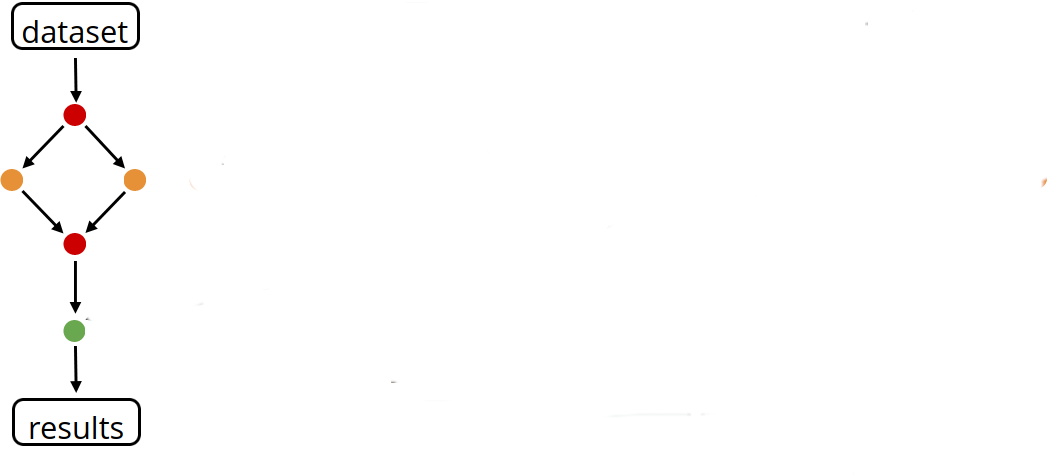
\includegraphics[width=0.7\textwidth]{Snakemake/analysis_1.png}};   
      \node at (7, 3.5) %[below=-0.4cm of analysis_1, xshift=2.7cm] at (current page.center)
         {
\includegraphics[width=0.45\textwidth]{Snakemake/phd_left.png}};
      \node at (6, 1) {\begin{minipage}{0.75\textwidth}\footnotesize
                        Idea from the official \lhref{https://slides.com/johanneskoester/snakemake-tutorial}{\Snakemake} course (with permission), image from \lhref{https://phdcomics.com/comics.php}{PhD comics}.
                       \end{minipage}
      };
    \end{tikzpicture}    
  \end{onlyenv}
  
  \begin{onlyenv}<2| handout:1>
    \begin{tikzpicture}
      \path[use as bounding box] (0.7,0) rectangle (12,8);
      \node[inner sep=0pt] (analysis_full) at (5,6)
         {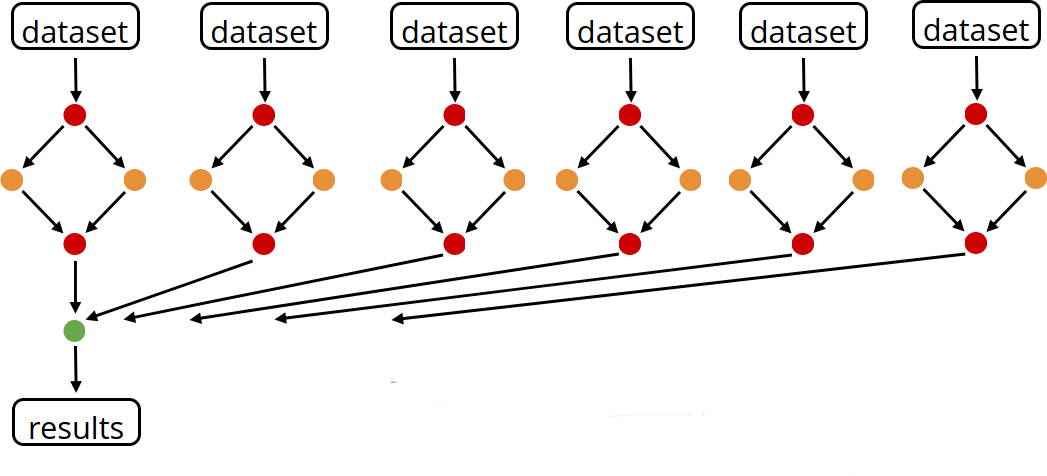
\includegraphics[width=0.7\textwidth]{Snakemake/analysis_full.png}};   
      \node at (7,3.5) % [below=-0.4cm of analysis_full, xshift=2.7cm]
         {
\includegraphics[width=0.45\textwidth]{Snakemake/phd_full.png}};
      \node at (6, 1) {\begin{minipage}{0.75\textwidth}\footnotesize
                        Idea from the official \lhref{https://slides.com/johanneskoester/snakemake-tutorial}{\Snakemake} course (with permission), image from \lhref{https://phdcomics.com/comics.php}{PhD comics}.
                       \end{minipage}
      };
    \end{tikzpicture}
  \end{onlyenv}
\end{frame}

%%%%%%%%%%%%%%%%%%%%%%%%%%%%%%%%%%%%%%%%%%%%%%%%%%%%%%%%%%%%%%%%%%%%%%%%%%%%%%%%
\begin{frame}
  \frametitle{Goals of Reproducibility}
  \Huge
  \begin{enumerate}
   \item Dispel Doubts
   \item Facilitate Further Experimentation
  \end{enumerate}
  \vfill
  \footnotesize{Idea from \lhref{https://elephly.net/downies/2023-dfn-slides.pdf}{DFN slides}.}
\end{frame}

%%%%%%%%%%%%%%%%%%%%%%%%%%%%%%%%%%%%%%%%%%%%%%%%%%%%%%%%%%%%%%%%%%%%%%%%%%%%%%%%
\begin{frame}
  \frametitle{Reproducible Data Analysis}
  \begin{onlyenv}<1| handout:0>
    \begin{tikzpicture}
      \path[use as bounding box] (0.7,0) rectangle (12,8);
      \node at (5.5, 5.5) {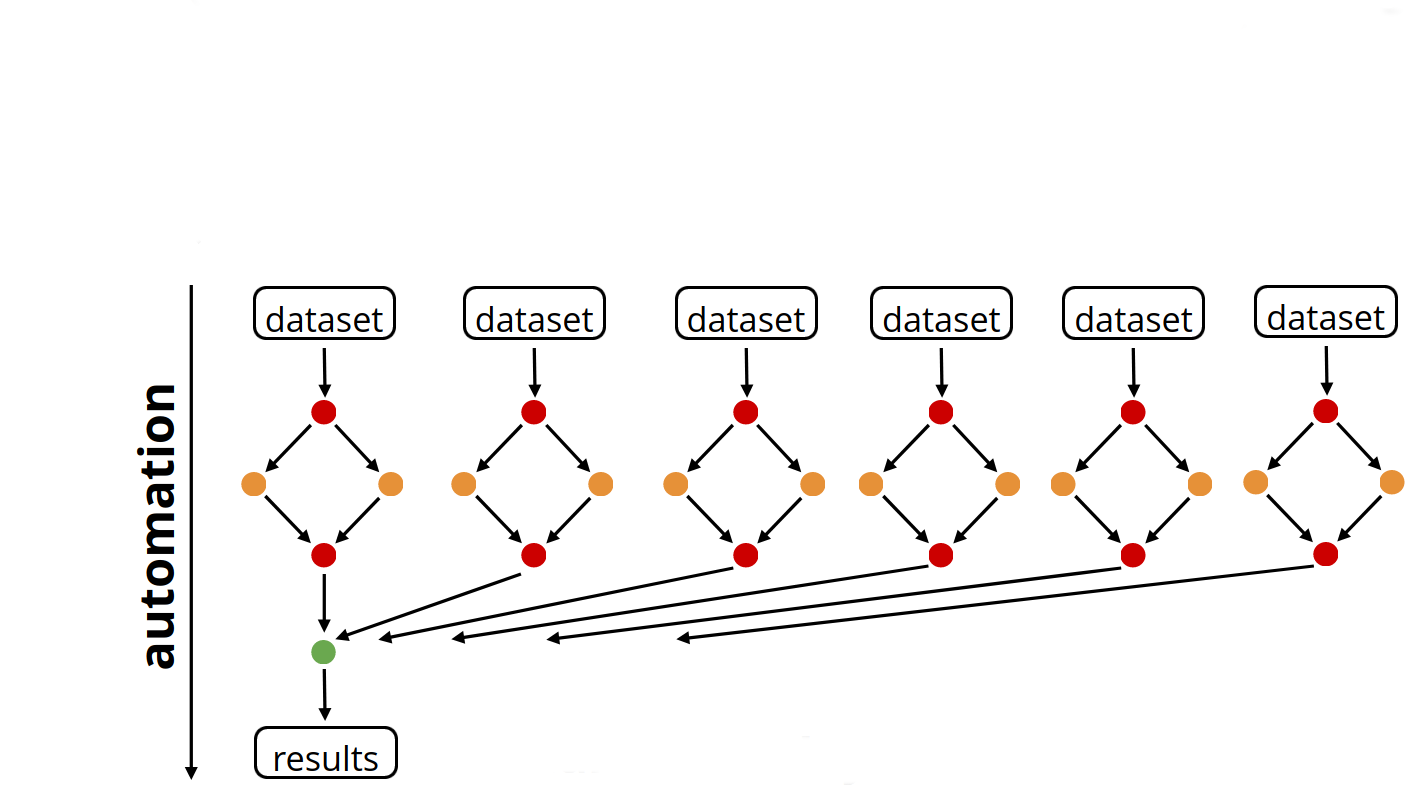
\includegraphics[width=0.7\textwidth]{Snakemake/automation.png}};
      \node at (8, 2.5) {\begin{minipage}{0.65\textwidth}
                             \textbf{From raw data to final figures:}
                             \begin{itemize}
                                \item \textbf{document} parameters, tools, versions
                                \item \textbf{execute} without manual intervention
                              \end{itemize}
                           \end{minipage}
                           };
    \end{tikzpicture}
  \end{onlyenv}
  \begin{onlyenv}<2| handout:0>
    \begin{tikzpicture}
      \path[use as bounding box] (0.7,0) rectangle (12,8);
      \node at (5.5, 5.5) {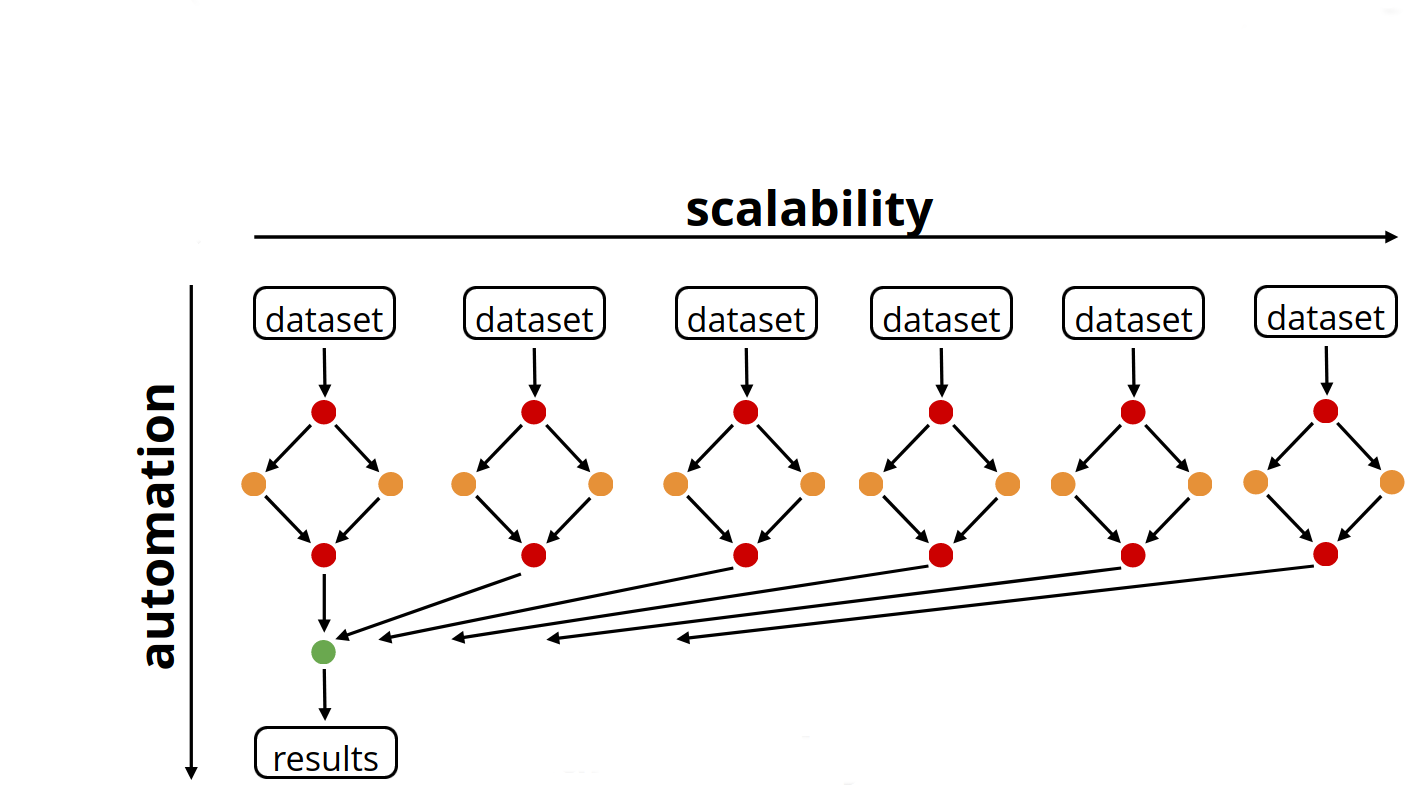
\includegraphics[width=0.7\textwidth]{Snakemake/scalability.png}};
      \node at (8, 2.5) {\begin{minipage}{0.65\textwidth}
                             \textbf{Handle parallelization:}
                             \begin{itemize}
                                \item execute for tens of thousands of datasets
                                \item efficiently use any computing platform
                              \end{itemize}
                           \end{minipage}
                           };
    \end{tikzpicture}
  \end{onlyenv}
  \begin{onlyenv}<3| handout:1>
    \begin{tikzpicture}
      \path[use as bounding box] (0.7,0) rectangle (12,8);
      \node at (5.5, 5.5) {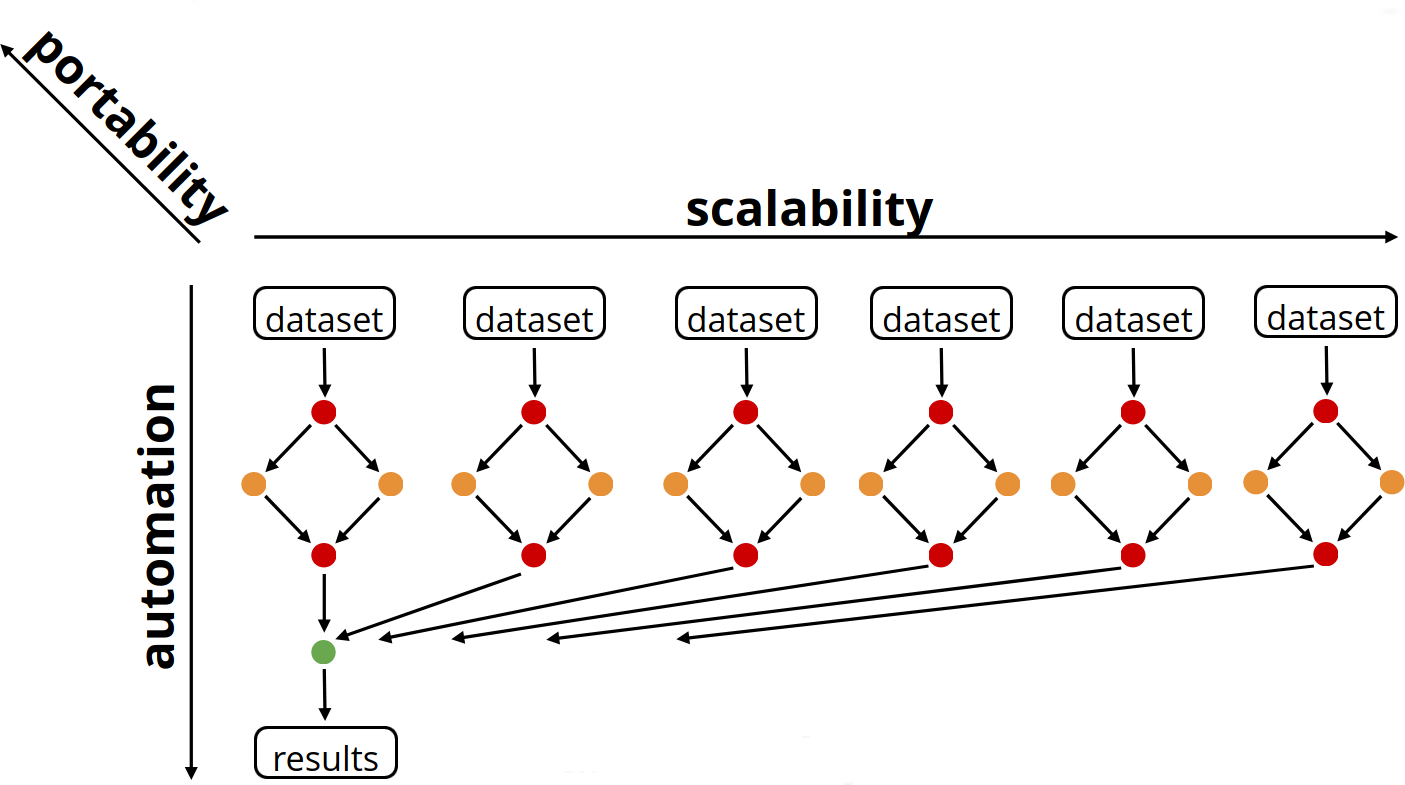
\includegraphics[width=0.7\textwidth]{Snakemake/portability.png}};
      \node at (8, 2.5) {\begin{minipage}{0.65\textwidth}
                             \textbf{Handle deployment:}\newline
                             be able to easily execute analyses on a different system/platform/infrastructure
                           \end{minipage}
                           };
    \end{tikzpicture}
  \end{onlyenv}
\end{frame}

%%%%%%%%%%%%%%%%%%%%%%%%%%%%%%%%%%%%%%%%%%%%%%%%%%%%%%%%%%%%%%%%%%%%%%%%%%%%%%%%
\begin{frame}
  \frametitle{Beyond Reproducibility}
  \begin{onlyenv}<1| handout:0>
    \begin{figure}
      \centering
      
\includegraphics[width=0.85\textwidth]{Snakemake/reproducibility_only.png}
    \end{figure}
  \end{onlyenv}
  \begin{onlyenv}<2| handout:0>
    \begin{figure}
      \centering
      
\includegraphics[width=0.85\textwidth]{Snakemake/reproducibility_empty.png}
    \end{figure}
  \end{onlyenv}
  \begin{onlyenv}<3| handout:0>
    \begin{figure}
      \centering
      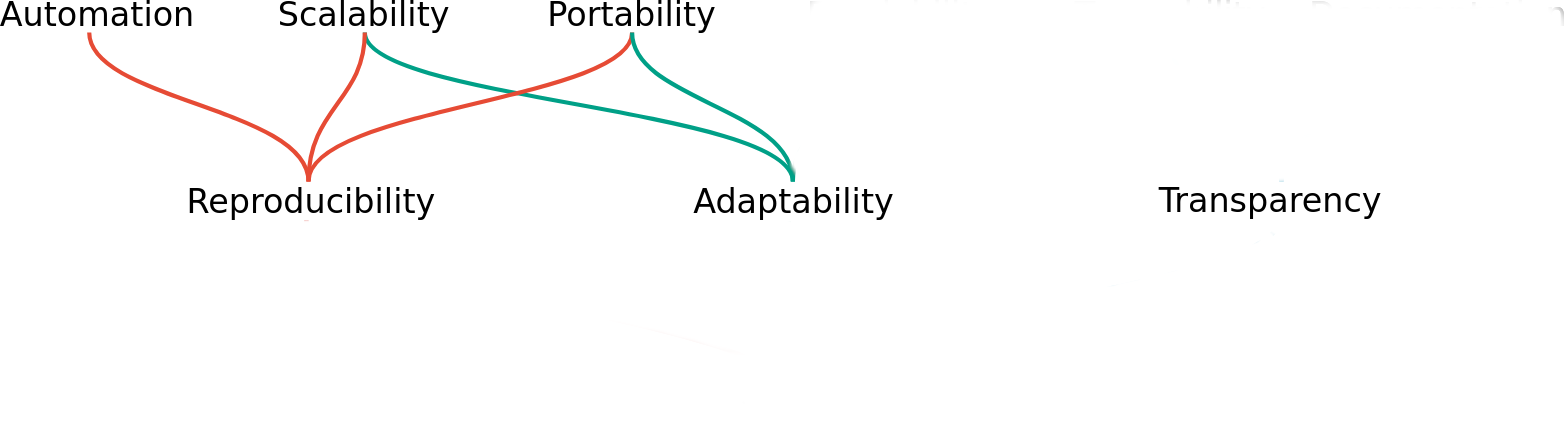
\includegraphics[width=0.85\textwidth]{Snakemake/reproducibility_left.png}
    \end{figure}
  \end{onlyenv}
    \begin{onlyenv}<4| handout:1>
      \begin{figure}
        \centering
        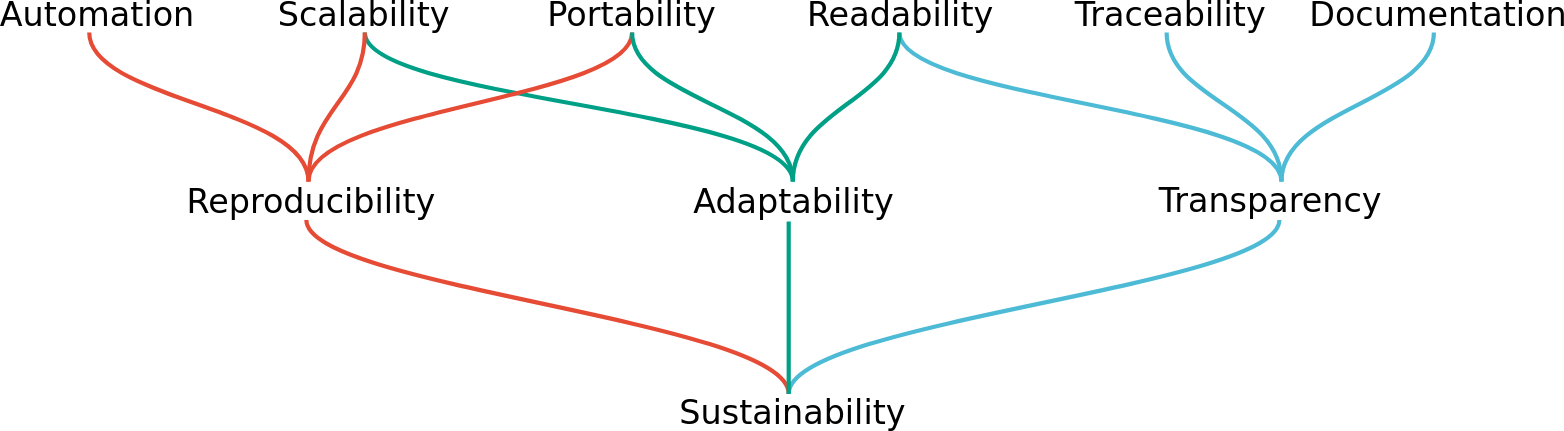
\includegraphics[width=0.85\textwidth]{Snakemake/reproducibility_full.png}
      \end{figure}
  \end{onlyenv}
  \footnotesize{\lhref{https://doi.org/10.12688/f1000research.29032.2}{From the official \Snakemake-paper.}}
\end{frame}


%%%%%%%%%%%%%%%%%%%%%%%%%%%%%%%%%%%%%%%%%%%%%%%%%%%%%%%%%%%%%%%%%%%%%%%%%%%%%%%%
\subsection{Goals, Background \& Outline}

%%%%%%%%%%%%%%%%%%%%%%%%%%%%%%%%%%%%%%%%%%%%%%%%%%%%%%%%%%%%%%%%%%%%%%%%%%%%%%%%
\begin{frame}
  \frametitle{Questions}
  \begin{question}[The questions you most probably have when starting your Analysis:]
  	\begin{itemize}
      \item How to start quickly (with the lowest amount of overhead)?
      \item What are the necessary tools?
    \end{itemize}
  \end{question}
                                                                               
  \begin{question}[Our question to you:]
  	 How do you get this information? And: Is reproducibility and sustainability your concern?
  \end{question}
  \pause
  \begin{block}{Most frequent Sources}
   \begin{itemize}
    \item Your labmate(s)
    \item The Internet
    \item Yes, of course ... eventually, when I brag about my paper/thesis.
   \end{itemize}
  \end{block}
\end{frame}

%%%%%%%%%%%%%%%%%%%%%%%%%%%%%%%%%%%%%%%%%%%%%%%%%%%%%%%%%%%%%%%%%%%%%%%%%%%%%%%%
\begin{frame}
  \frametitle{The Workflow Approach}
  Workflow Engines answer these questions directly by providing
  \begin{itemize}
   \item entire Workflows can be selected and can be put to action.
   \item executing routines reliably.
  \end{itemize}
\end{frame}

%%%%%%%%%%%%%%%%%%%%%%%%%%%%%%%%%%%%%%%%%%%%%%%%%%%%%%%%%%%%%%%%%%%%%%%%%%%%%%%%
\begin{frame}
  \frametitle{Going HPC}
  \begin{question}
  	Why would you want to work on a cluster?
  \end{question}
  \pause
  Answers may include:
  \begin{itemize}[<+->]
   \item compute power and ressources for big data
   \item launching scalable (and otherwise portable) workflows with workflow engines
  \end{itemize}
\end{frame}


%%%%%%%%%%%%%%%%%%%%%%%%%%%%%%%%%%%%%%%%%%%%%%%%%%%%%%%%%%%%%%%%%%%%%%%%%%%%%%%%
%%%%%%%%%%%%%%%%%%%%%%%%%%%%%%%%%%%%%%%%%%%%%%%%%%%%%%%%%%%%%%%%%%%%%%%%%%%%%%%%
\section{Software Environment}

%%%%%%%%%%%%%%%%%%%%%%%%%%%%%%%%%%%%%%%%%%%%%%%%%%%%%%%%%%%%%%%%%%%%%%%%%%%%%%%%
\begin{frame}
	\frametitle{Outline}
	\begin{columns}[t]
		\begin{column}{.5\textwidth}
            \tableofcontents[sections={1-7},currentsection]
		\end{column}
		\begin{column}{.5\textwidth}
            \tableofcontents[sections={8-15},currentsection]
		\end{column}
	\end{columns}
\end{frame}

%%%%%%%%%%%%%%%%%%%%%%%%%%%%%%%%%%%%%%%%%%%%%%%%%%%%%%%%%%%%%%%%%%%%%%%%%%%%%%%%
\begin{frame}
	\frametitle{What is this about?}
	\begin{question}[Questions]\begin{itemize}
			\item How do I get the software for a particular workflow?
			\item What is the difference in different build systems and software environments? Why does it matter for me?
		\end{itemize}
	\end{question}
	\begin{docs}[Objectives]
	  \begin{enumerate}
			\item Introducing the "Module" system provided on HPC clusters (briefly).
			\item Learning how to install software with "Conda".
			\item Knowing how to avoid conflicts between the different software provisioning schemes.
	  \end{enumerate}
    \end{docs}
\end{frame}

%%%%%%%%%%%%%%%%%%%%%%%%%%%%%%%%%%%%%%%%%%%%%%%%%%%%%%%%%%%%%%%%%%%%%%%%%%%%%%%%
\subsection{Software on HPC Systems}

%%%%%%%%%%%%%%%%%%%%%%%%%%%%%%%%%%%%%%%%%%%%%%%%%%%%%%%%%%%%%%%%%%%%%%%%%%%%%%% 
\begin{frame}
  \frametitle{Modules}
  \vspace{-1.3em}
  \begin{block}{What is a module?}
    A module collects all environment variables and settings needed for a particular software package (e.\,g. path to executable and libraries).
  \end{block}

  \vfill
\end{frame}

%TODO: discuss: is this too dense? This works for lmod (see next slide on the spider command). Too specific?
%%%%%%%%%%%%%%%%%%%%%%%%%%%%%%%%%%%%%%%%%%%%%%%%%%%%%%%%%%%%%%%%%%%%%%%%%%%%%%%
\begin{frame}[fragile]
  {Modules -- Command Overview}
  \vspace{-1em}
  \begin{itemize}
    \setlength\itemsep{-0.1em}
  \item List of all available modules
    \begin{lstlisting}[language=Bash, style=Shell]
$ module avail             # or 'module av'
    \end{lstlisting}
  \item Loading a specific module
    \begin{lstlisting}[language=Bash, style=Shell]
$ module load <modulename> # or 'module add'
    \end{lstlisting}
  \item Showing all currently loaded modules
    \begin{lstlisting}[language=Bash, style=Shell]
$ module list
    \end{lstlisting}
  \item Unloading a specific module
    \begin{lstlisting}[language=Bash, style=Shell]
$ module unload <modulename>
    \end{lstlisting}
  \item Unload all active modules
    \begin{lstlisting}[language=Bash, style=Shell]
$ module purge
    \end{lstlisting}
  \end{itemize}
  \vfill
\end{frame}

%%%%%%%%%%%%%%%%%%%%%%%%%%%%%%%%%%%%%%%%%%%%%%%%%%%%%%%%%%%%%%%%%%%%%%%%%%%%%%%
\begin{frame}[fragile]
  \frametitle{Modules -- looking for specific modules}
  Looking up modules:
  \begin{lstlisting}[language=Bash, style=Shell]
$ module spider <search string>
  \end{lstlisting}
  \pause
  \begin{task}[Looking for area specific modules]
  	Try looking for an area specific 
    module, e.\,g. in ``\texttt{bwa}''
  \end{task}
\end{frame}

%%%%%%%%%%%%%%%%%%%%%%%%%%%%%%%%%%%%%%%%%%%%%%%%%%%%%%%%%%%%%%%%%%%%%%%%%%%%%%%
\begin{frame}[fragile]
  \frametitle{Module Naming Schemes}
   You might have seen module names like:
   \begin{lstlisting}[language=Bash, style=Shell]
numlib/FFTW/3.3.10-gompi-2021b   
   \end{lstlisting}
   Actual module naming schemes differ from cluster to cluster.
   \pause
   \begin{block}{Using Modules with \Snakemake{}}
     We will learn how to use modules with 
   \end{block}
   \pause
   \begin{task}[Look inside a module to know what will be loaded and set]
   	  Do ``\altverb{module show <module>}''
   \end{task}
\end{frame}

%%%%%%%%%%%%%%%%%%%%%%%%%%%%%%%%%%%%%%%%%%%%%%%%%%%%%%%%%%%%%%%%%%%%%%%%%%%%%%% 
\begin{frame}[fragile]
  \frametitle{That's all Folks}
   \vspace{-0.8em}
  \begin{alertblock}{Why we will not go in depth now}
You can learn more about modules in 101-HPC courses. Later, we will learn how to use \Snakemake{} workflows, particularly curated ones, available on the web. We \emph{could} re-write and adapt them for a specific cluster, it is better to only parameterize them and do leave the workflow itself unaltered, portable. This is less cumbersome and as workflow systems, including \Snakemake{}, rely on Conda, we will have an in-depth intro to Conda, instead.
  \end{alertblock}
  \vfill
  \begin{alertblock}{Do not mix Conda with Modules}
   Do not mix Conda with module files - particularly, avoid writing \altverb{module load} commands in your \texttt{\textasciitilde/.bashrc} file.\newline
   Whenever your modules or Conda are using conflicting compilers or environments, you might not be able to execute your software or -- \emph{worse} -- will result in funny crashes with apparently no reason.
  \end{alertblock}
\end{frame}

%%%%%%%%%%%%%%%%%%%%%%%%%%%%%%%%%%%%%%%%%%%%%%%%%%%%%%%%%%%%%%%%%%%%%%%%%%%%%%% 
\subsection{Using Conda}

%%%%%%%%%%%%%%%%%%%%%%%%%%%%%%%%%%%%%%%%%%%%%%%%%%%%%%%%%%%%%%%%%%%%%%%%%%%%%%% 
\begin{frame}<handout:0> 
  \frametitle{Your Work Environment with Conda}
  \begin{columns}
    \begin{column}{0.5\textwidth}\centering
      
\includegraphics[width=0.8\textwidth]{environment/environment.png}
    \end{column}
    \begin{column}{0.5\textwidth}\centering
      
\includegraphics[width=0.8\textwidth]{logos/Conda_logo.png}   
    \end{column}
  \end{columns}
\end{frame}

%%%%%%%%%%%%%%%%%%%%%%%%%%%%%%%%%%%%%%%%%%%%%%%%%%%%%%%%%%%%%%%%%%%%%%%%%%%%%%% 
\begin{frame}
  \frametitle{Conda vs. Module Files}
  \begin{columns}
    \begin{column}{0.5\textwidth}
      Background Module Files
      \begin{itemize}
       \item module files provide an environment per software
       \item the software usually is compiled on the machine (optimized)
       \item due to differences in cluster naming schemes and setups portability cannot be granted
      \end{itemize}
    \end{column}
    \begin{column}{0.5\textwidth}
      Background Conda
      \begin{itemize}
       \item Conda is a machine independent package management systems
       \item packaged software is provided pre-compiled (NOT optimized)
       \item Conda allows for grouping software stacks in environments, therefore ensuring portability
      \end{itemize}
    \end{column}
  \end{columns}
\end{frame}


%%%%%%%%%%%%%%%%%%%%%%%%%%%%%%%%%%%%%%%%%%%%%%%%%%%%%%%%%%%%%%%%%%%%%%%%%%%%%%% 
\begin{frame}[fragile]
  \frametitle{Installing Conda}
  You \emph{could} run
  \begin{lstlisting}[language=Bash, style=Shell, basicstyle=\small,breaklines=true ]
$ wget https://repo.anaconda.com/miniconda/Miniconda3-latest-Linux-x86_64.sh
  \end{lstlisting}
  to retrieve (Mini)Conda (a flavour of conda with less overhead).
  \begin{hint}
  	\footnotesize URL is from \url{https://docs.conda.io/en/latest/miniconda.html}.\newline However, we are going to use tweaked scripts provided to you.
  \end{hint}
  \pause
  \begin{hint}
  	However, instead of downloading, we will work through this together on the slides to come.
  \end{hint}
\end{frame} 

%%%%%%%%%%%%%%%%%%%%%%%%%%%%%%%%%%%%%%%%%%%%%%%%%%%%%%%%%%%%%%%%%%%%%%%%%%%%%%% 
\begin{frame}[fragile]
  \frametitle{We will favour \emph{\textmu-Mamba} over Conda!}
  Many know ``Conda'' as a package manager -- and this is correct! But:
  \begin{block}{Why we recommend using ``\textmu-Mamba''}
   Conda carries some overhead. Alternative implementations can be faster and require less files. Mamba is a ``drop-in'' for Conda. This means: \emph{every command is the same}, except we will write \altverb{mamba} where usuall \altverb{conda} would be.\newline
   Why?\newline
   Mamba is an implementation of Conda, written in \CC{}. It is able to carry out some tasks in parallel and works considerably faster. In turn, \textmu-Mamba is a staticically compiled version of Mamba and does not require a ``base'' environment (we will learn about environments, soon), which means even less overhead.
  \end{block}
\end{frame}

%%%%%%%%%%%%%%%%%%%%%%%%%%%%%%%%%%%%%%%%%%%%%%%%%%%%%%%%%%%%%%%%%%%%%%%%%%%%%%% 
\begin{frame}[fragile]
	\frametitle{Installing \sout{Conda}/\textmu-Mamba}
	Please run
	\begin{lstlisting}[language=Bash, style=Shell]
$ "${SHELL}" <(curl -L micro.mamba.pm/install.sh)
	\end{lstlisting}
\end{frame}

%%%%%%%%%%%%%%%%%%%%%%%%%%%%%%%%%%%%%%%%%%%%%%%%%%%%%%%%%%%%%%%%%%%%%%%%%%%%%%%% 
\begin{frame}
  \frametitle{Installing \sout{Conda}/\textmu-Mamba - II}
  You need to confirm (with ``Enter'')
  \begin{itemize}[<+->]
	\item the binary folder.
	\item the shell you are using (just to be on the save side)
	\item whether conda-forge shall be configured (this is a major resource channel)
	\item the prefix location (where \textmu-Mamba shall be placed)
  \end{itemize} 
  The tool will tell up about the modification of your \altverb{.bashrc} file (which is executed upon \emph{every} login, we will discuss this in a minute).
\end{frame}
	
%%%%%%%%%%%%%%%%%%%%%%%%%%%%%%%%%%%%%%%%%%%%%%%%%%%%%%%%%%%%%%%%%%%%%%%%%%%%%%% 
\begin{frame}[fragile]
  \frametitle{Installing \sout{Conda}/\textmu-Mamba - III}
  \footnotesize
  \begin{columns}[t]
    \begin{column}{0.5\textwidth}
       You now have a section like this in your ``\texttt{\textasciitilde/.bashrc}'':
       \begin{lstlisting}[language=Bash, style=Shell, basicstyle=\tiny, breaklines=true]
# >>> mamba initialize >>>
# !! Contents within this block are managed by 'mamba init' !!
export MAMBA_EXE='/home/cm/.local/bin/micromamba';
export MAMBA_ROOT_PREFIX='/home/cm/micromamba';
__mamba_setup="$("$MAMBA_EXE" shell hook --shell bash --root-prefix "$MAMBA_ROOT_PREFIX" 2> /dev/null)"
if [ $? -eq 0 ]; then
    eval "$__mamba_setup"
else
    alias micromamba="$MAMBA_EXE"  # Fallback on help from mamba activate
fi
unset __mamba_setup
# <<< mamba initialize <<<
      \end{lstlisting}
      \bcattention \emph{Every} time you log-in this will be executed. Also, here, ``\texttt{<prefix>}'' denotes \emph{your} prefix.
    \end{column}
    \begin{column}{0.5\textwidth}
       \pause
       Please edit your ``\texttt{\textasciitilde/.bashrc}'' file and put part in a function, to re-gain manual control:
       \begin{lstlisting}[language=Bash, style=Shell, basicstyle=\tiny, breaklines=true]
@function conda_initialize {@
# >>> mamba initialize >>>
# !! Contents within this block are managed by 'mamba init' !!
export MAMBA_EXE='/home/cm/.local/bin/micromamba';
export MAMBA_ROOT_PREFIX='/home/cm/micromamba';
__mamba_setup="$("$MAMBA_EXE" shell hook --shell bash --root-prefix "$MAMBA_ROOT_PREFIX" 2> /dev/null)"
if [ $? -eq 0 ]; then
    eval "$__mamba_setup"
else
    alias micromamba="$MAMBA_EXE"  # Fallback on help from mamba activate
fi
unset __mamba_setup
# <<< mamba initialize <<<
@}@
      \end{lstlisting}
      \bcattention Add the highlighted lines! and your login will be faster! Also, this allows to separate the module environment and conda-related environments safely.
    \end{column}
  \end{columns}
\end{frame}


%%%%%%%%%%%%%%%%%%%%%%%%%%%%%%%%%%%%%%%%%%%%%%%%%%%%%%%%%%%%%%%%%%%%%%%%%%%%%% 
\begin{frame}[fragile]
  \frametitle{Why this function in your \texttt{.bashrc}?}
  \begin{docs}
  	\begin{itemize}[<+->]
  		\item \emph{every} time you log in, the code in your \texttt{.bashrc} will be exectud. Depeding on your conda setup, this can be incredibly slow (another reason to use Mamba or \textmu-Mamba).
  		\item automatic inclusion of Conda/Mamba might cause interference with modules
  		\item Now, you can run \verb+conda_initialize+ in the login shell, jobs scripts, etc. upon demand and deactivate if needed.
  	\end{itemize}
  \end{docs}
\end{frame}

%%%%%%%%%%%%%%%%%%%%%%%%%%%%%%%%%%%%%%%%%%%%%%%%%%%%%%%%%%%%%%%%%%%%%%%%%%%%%%% 
\begin{frame}[fragile]
  \frametitle{Initializing Conda \& Mamba}
  To initialize Conda, simply run
  \begin{lstlisting}[language=Bash, style=Shell]
$ bash
  \end{lstlisting}
  or (better)
  \begin{lstlisting}[language=Bash, style=Shell]
$ source ~/.bashrc
  \end{lstlisting}
  Subsequently, run: 
  \begin{lstlisting}[language=Bash, style=Shell]
$ conda_initialize # if you have this function
  \end{lstlisting}
\end{frame}

%%%%%%%%%%%%%%%%%%%%%%%%%%%%%%%%%%%%%%%%%%%%%%%%%%%%%%%%%%%%%%%%%%%%%%%%%%%%%%% 
\input{\configparam{condarcfile}}

%%%%%%%%%%%%%%%%%%%%%%%%%%%%%%%%%%%%%%%%%%%%%%%%%%%%%%%%%%%%%%%%%%%%%%%%%%%%%%% 
\begin{frame}[fragile]
  \frametitle{Searching Software with Conda v. Mamba}
  First you might want to look for software. This is done with
  \begin{lstlisting}[language=Bash, style=Shell]
$ micromamba search <softwarename>
  \end{lstlisting}
  \pause
  \begin{task}
  	Try this with a software which comes to mind.
  \end{task}
  \pause
  This will list packages with channel and version information, e.\,g.
  \begin{lstlisting}[language=Bash, style=Shell, basicstyle=\tiny]
$ micromamba search minimap
<snip>
Loading channels: done
# Name                       Version           Build  Channel             
minimap                     0.2_r124               0  bioconda            
minimap                     0.2_r124      h5bf99c6_4  bioconda
....
  \end{lstlisting}
\end{frame}


%%%%%%%%%%%%%%%%%%%%%%%%%%%%%%%%%%%%%%%%%%%%%%%%%%%%%%%%%%%%%%%%%%%%%%%%%%%%%%% 
\begin{frame}
  \frametitle{Installing Software \emph{with} Conda \& Mamba - Using Environments}
  \begin{hint}It is a good habit to have
        \begin{itemize}
          \item \emph{one} environment per workflow
          \item the environment named as the workflow
          \item this way, we have a bundle of tools, activate the environment for it
          \item \Snakemake{} workflows will install the tools you need for a particular workflow - only \emph{if} these tools are still missing
         \end{itemize}
  \end{hint}
  \begin{hint}[Note]
  	For now we will not use \Snakemake{} to install our software. This topic will be covered later.
  \end{hint}
\end{frame}

%%%%%%%%%%%%%%%%%%%%%%%%%%%%%%%%%%%%%%%%%%%%%%%%%%%%%%%%%%%%%%%%%%%%%%%%%%%%%%% 
\begin{frame}[fragile]
  \frametitle{Conda / Mamba Environments}
  With Conda/Mamba, we can activate and deactivate environments, which bundle our software. E.\,g. a software stack per workflow to ensure reproducible runs.
    \pause
  To generate a new we can run
  \begin{lstlisting}[language=Bash, style=Shell]
$ micromamba create @-n@ <environment_name>
  \end{lstlisting}
  This will create a new environment with a given name in your home directory. Alternatively, i.\,e. when dealing with file number quotas, you can point the environment to a different filesystem, e.\,g.:
  \begin{lstlisting}[language=Bash, style=Shell] 
$ micromamba create \
>  @-p@ /path/to/project/fs/<environment_name>
   \end{lstlisting}
\end{frame}

%%%%%%%%%%%%%%%%%%%%%%%%%%%%%%%%%%%%%%%%%%%%%%%%%%%%%%%%%%%%%%%%%%%%%%%%%%%%%%% 
\begin{frame}[fragile]
  \frametitle{\HandsOn{Creating your own Environment}}
  Now, create your first environment. We will
  \begin{itemize}
  	\item work in the \altverb{snakemake_tutorial} directory with
  	\item a \textit{named} environment
  	\item use the downloaded \altverb{environment.yaml} file to define the software stack
  	\item pre-compile all Python files with the \altverb{--pyc} flag
  \end{itemize}
  \begin{lstlisting}[language=Bash, style=Shell,breaklines=true]
$ micromamba create --pyc -f environment.yaml -n snakemake-tutorial
  \end{lstlisting}	
\end{frame}

%%%%%%%%%%%%%%%%%%%%%%%%%%%%%%%%%%%%%%%%%%%%%%%%%%%%%%%%%%%%%%%%%%%%%%%%%%%%%%% 
\begin{frame}[fragile]
  \frametitle{Listing Environments}
   Over time you will have several environments. (So far, there is one.) To list them all, simply run:
  \begin{lstlisting}[language=Bash, style=Shell]
$ micromamba env list
  \end{lstlisting}
\end{frame} 

%%%%%%%%%%%%%%%%%%%%%%%%%%%%%%%%%%%%%%%%%%%%%%%%%%%%%%%%%%%%%%%%%%%%%%%%%%%%%%% 
\begin{frame}[fragile]
  \frametitle{Creating, Activating, Deactivating Environments}
  We can create, activate and deactivate environments with
  \begin{lstlisting}[language=Bash, style=Shell]
$ micromamba create [other args] -n <environment name>
$ micromamba activate <environment name>
$ micromamba deactivate
  \end{lstlisting}
   \begin{task}
   	  Activate the environment you just created!
   \end{task}
\end{frame}

%%%%%%%%%%%%%%%%%%%%%%%%%%%%%%%%%%%%%%%%%%%%%%%%%%%%%%%%%%%%%%%%%%%%%%%%%%%%%%% 
\begin{frame}[fragile]
   \frametitle{\Interlude{Managing your Prompt}}
   \begin{question}
   	Did you notice the last line in your \texttt{.condarc} file? What does it do?
   \end{question} 
   Remember:
     \begin{lstlisting}[language=Bash, style=Shell]
$ cat .condarc
....
env_prompt: '($(basename {default_env})) '
   \end{lstlisting}
   \pause
   It causes an unnamed environment prompt to shrink, e.\,g.:
   \begin{lstlisting}[language=Bash, style=Plain]
(my_env) user@host:directory $
# instead of
(/some/long/path/my_env) user@host:directory $
   \end{lstlisting}
\end{frame}





%%%%%%%%%%%%%%%%%%%%%%%%%%%%%%%%%%%%%%%%%%%%%%%%%%%%%%%%%%%%%%%%%%%%%%%%%%%%%%%%
%\section{Selecting curated Workflows}

%%%%%%%%%%%%%%%%%%%%%%%%%%%%%%%%%%%%%%%%%%%%%%%%%%%%%%%%%%%%%%%%%%%%%%%%%%%%%%%%
\begin{frame}
    \frametitle{Outline}
    \begin{columns}[t]
        \begin{column}{.5\textwidth}
            \tableofcontents[sections={1-9},currentsection]
        \end{column}
        \begin{column}{.5\textwidth}
            \tableofcontents[sections={10-18},currentsection]
        \end{column}
    \end{columns}
\end{frame}


%%%%%%%%%%%%%%%%%%%%%%%%%%%%%%%%%%%%%%%%%%%%%%%%%%%%%%%%%%%%%%%%%%%%%%%%%%%%%%%%
\begin{frame}
  \frametitle{What is this about?}
   \question[Questions]{\begin{itemize}
                         \item How do I get a workflow for a given scientific problem?
                         \item How do I run such an arbitrary workflow?
                        \end{itemize}
                       }
   \docs[Objectives]{\begin{enumerate}
                      \item Introducing the worfkflow catalogue?
                      \item Learning the difference between ``curation'' (what some people think) and ``curation'' (what really works)?
                     \end{enumerate}}
\end{frame}  

\subsection{The \texttt{Snakemake} Workflow Catalogue}

%%%%%%%%%%%%%%%%%%%%%%%%%%%%%%%%%%%%%%%%%%%%%%%%%%%%%%%%%%%%%%%%%%%%%%%%%%%%%%%%
\begin{frame}
 \frametitle{Selecting and Downloading from the Workflow Catalogue}
 You can find the \texttt{Snakemake} worfkflow catalogue, \lhref{https://snakemake.github.io/snakemake-workflow-catalog/?rules=true}{here}. It makes a difference between workflows which meet best-practice criteria - and those which do not.\newline
 \begin{columns}
   \begin{column}{0.5\textwidth}
     You can download and run any workflow. \pause\newline
     \warning{Except, you most likely cannot, because of a missing cluster configuration and some missing features.}
   \end{column}
   \begin{column}{0.5\textwidth}
     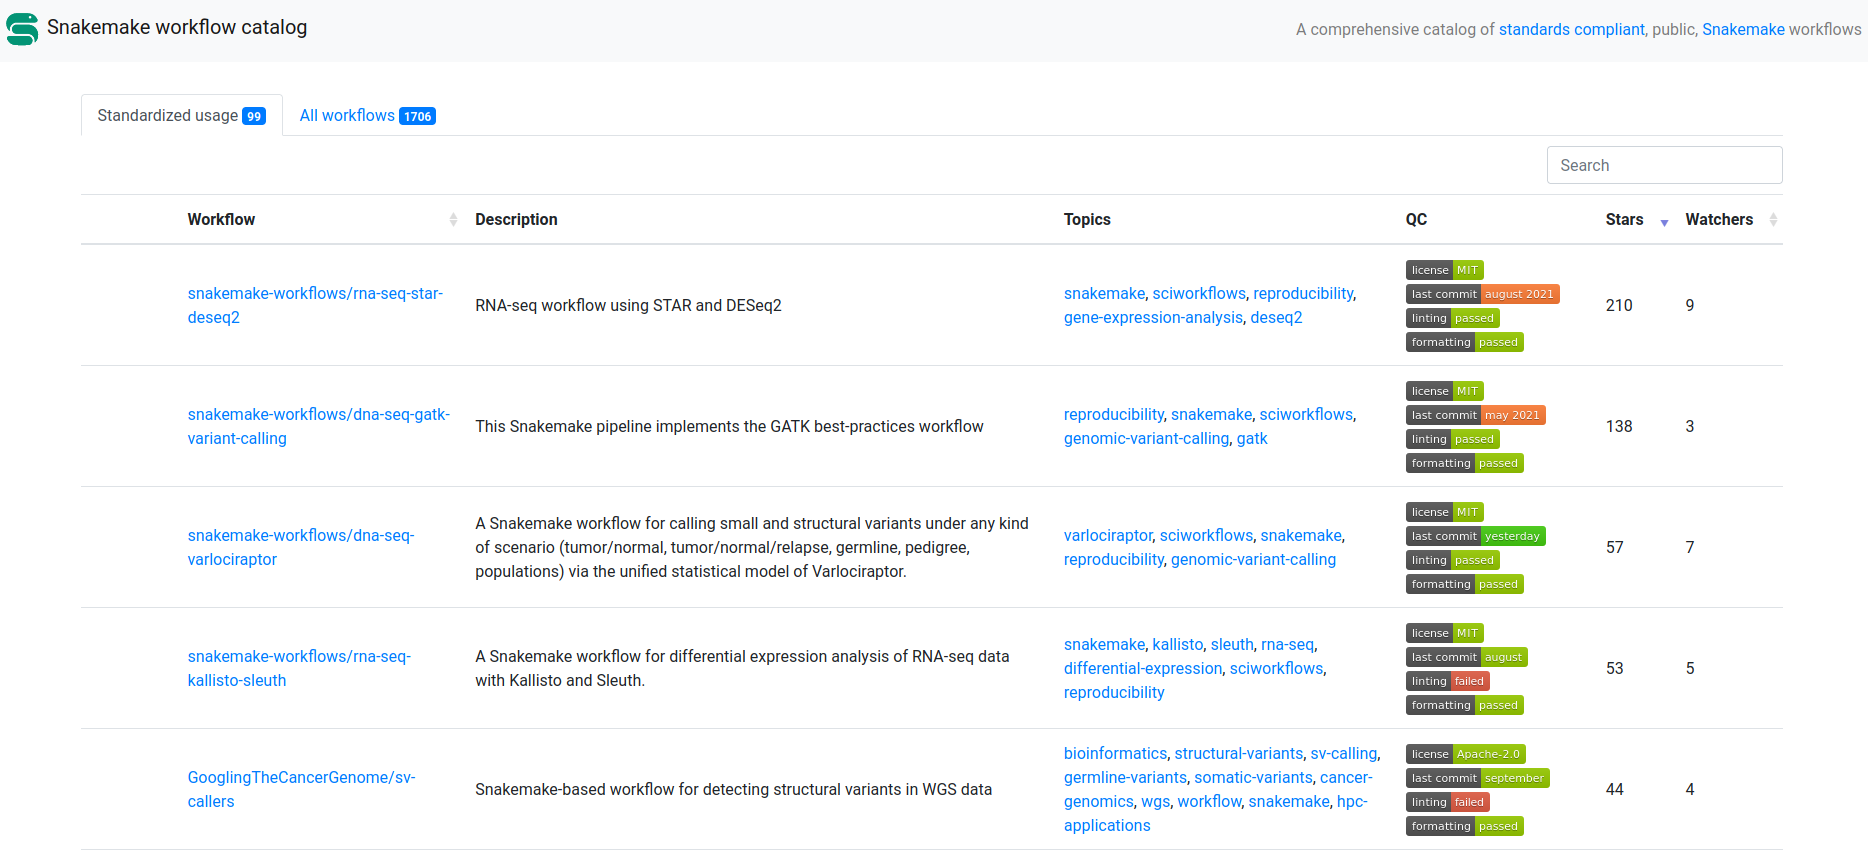
\includegraphics[width=\textwidth]{Snakemake/Snakemake_Workflow_Catalog.png}
   \end{column}
 \end{columns}
\end{frame}

%%%%%%%%%%%%%%%%%%%%%%%%%%%%%%%%%%%%%%%%%%%%%%%%%%%%%%%%%%%%%%%%%%%%%%%%%%%%%%%%
\begin{frame}[fragile]
  \frametitle{Deployment}
  Select (=click on) any desired workflow. There are two alternatives:
  \begin{enumerate}
   \item a workflow offeres a release - in which case you can download and unpack it
   \item all workflows offers a ``\altverb{git clone}'' hint
  \end{enumerate}
\end{frame}

%%%%%%%%%%%%%%%%%%%%%%%%%%%%%%%%%%%%%%%%%%%%%%%%%%%%%%%%%%%%%%%%%%%%%%%%%%%%%%%%
\begin{frame}[fragile]
  \frametitle{Running Workflows on Cluster (or other environment)}
  Most likely a specific workflow never has been testing on \emph{your} computer before. It is almost ensured it will run on arbitrary servers, but clusters are a different story. \newline
  So
  \begin{itemize}[<+->]
   \item try to parameterize your workflow as learned
   \item if it gives issues and you know how to correct it, ``fork'' the worklow and create a pull request
   \item if you cannot fix it, create a bug report
  \end{itemize}
\end{frame}

%%%%%%%%%%%%%%%%%%%%%%%%%%%%%%%%%%%%%%%%%%%%%%%%%%%%%%%%%%%%%%%%%%%%%%%%%%%%%%%%
\begin{frame}
  \frametitle{\Interlude{Learn git!}}
  If you do not know what ``fork'' and ``pull request'' means, learn git!
  \begin{itemize}[<+->]
   \item there are courses
   \item and lots of online material
   \item and books
  \end{itemize}
  \pause
  \warning{Knowing git is essential in data analysis!}
\end{frame}




%%%%%%%%%%%%%%%%%%%%%%%%%%%%%%%%%%%%%%%%%%%%%%%%%%%%%%%%%%%%%%%%%%%%%%%%%%%%%%%%
%\include{common/Using_Workflow_Configs}

%%%%%%%%%%%%%%%%%%%%%%%%%%%%%%%%%%%%%%%%%%%%%%%%%%%%%%%%%%%%%%%%%%%%%%%%%%%%%%%%
%%%%%%%%%%%%%%%%%%%%%%%%%%%%%%%%%%%%%%%%%%%%%%%%%%%%%%%%%%%%%%%%%%%%%%%%%%%%%%%%
\section{Plotting DAGs}

%%%%%%%%%%%%%%%%%%%%%%%%%%%%%%%%%%%%%%%%%%%%%%%%%%%%%%%%%%%%%%%%%%%%%%%%%%%%%%%%
\begin{frame}
    \frametitle{Outline}
    \begin{columns}[t]
        \begin{column}{.5\textwidth}
            \tableofcontents[sections={1-9},currentsection]
        \end{column}
        \begin{column}{.5\textwidth}
            \tableofcontents[sections={10-18},currentsection]
        \end{column}
    \end{columns}
\end{frame}

%%%%%%%%%%%%%%%%%%%%%%%%%%%%%%%%%%%%%%%%%%%%%%%%%%%%%%%%%%%%%%%%%%%%%%%%%%%%%%%%
\begin{frame}
  \frametitle{What is this about?}
   \question[Questions]{\begin{itemize}
                         \item How do we plot our workflows for a publication?
                        \end{itemize}
                       }
   \docs[Objectives]{\begin{enumerate} 
                      \item Learn to plot workflows using \texttt{Snakemake} and \texttt{GraphViz}.
                     \end{enumerate}}
\end{frame}


%%%%%%%%%%%%%%%%%%%%%%%%%%%%%%%%%%%%%%%%%%%%%%%%%%%%%%%%%%%%%%%%%%%%%%%%%%%%%%%%
\begin{frame}[fragile]
  \frametitle{\HandsOn{Plotting the Workflow}}
  \texttt{Snakemake} has a build-in plotting feature. Run 
  \begin{lstlisting}[language=Bash, style=Shell]
$ snakemake --rulegraph | dot -Tpng > <your_workflow.png>
  \end{lstlisting}
  to plot your workflow graph. And
  \begin{lstlisting}[language=Bash, style=Shell]
$ display <your_workflow.png>
  \end{lstlisting}
  to display the workflow.
\end{frame}

%%%%%%%%%%%%%%%%%%%%%%%%%%%%%%%%%%%%%%%%%%%%%%%%%%%%%%%%%%%%%%%%%%%%%%%%%%%%%%%%
\begin{frame}
  \frametitle{Your DAG:}
  \centering
  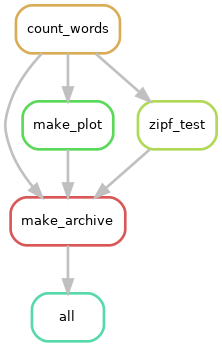
\includegraphics[width=0.4\textwidth]{workflows/complete_workflow.png}
\end{frame}


%%%%%%%%%%%%%%%%%%%%%%%%%%%%%%%%%%%%%%%%%%%%%%%%%%%%%%%%%%%%%%%%%%%%%%%%%%%%%%%%
%%%%%%%%%%%%%%%%%%%%%%%%%%%%%%%%%%%%%%%%%%%%%%%%%%%%%%%%%%%%%%%%%%%%%%%%%%%%%%%%
\section{How does Clustercomputing work?}

%%%%%%%%%%%%%%%%%%%%%%%%%%%%%%%%%%%%%%%%%%%%%%%%%%%%%%%%%%%%%%%%%%%%%%%%%%%%%%%%
\begin{frame}
    \frametitle{Outline}
    \begin{columns}[t]
        \begin{column}{.5\textwidth}
            \tableofcontents[sections={1-9},currentsection]
        \end{column}
        \begin{column}{.5\textwidth}
            \tableofcontents[sections={10-18},currentsection]
        \end{column}
    \end{columns}
\end{frame}

%%%%%%%%%%%%%%%%%%%%%%%%%%%%%%%%%%%%%%%%%%%%%%%%%%%%%%%%%%%%%%%%%%%%%%%%%%%%%%%%
\begin{frame}
  \frametitle{What is this about?}
    \begin{question}
   	  \begin{itemize}
        \item How does ordinary job submission work on a cluster?
        \item How does it work using Snakemake? (Which parameterization is necessary?)
      \end{itemize}
   \end{question}
   \docs[Objectives]{\begin{enumerate} 
                      \item Get a feeling for the SLURM batch system.
                     \end{enumerate}}
\end{frame}


%%%%%%%%%%%%%%%%%%%%%%%%%%%%%%%%%%%%%%%%%%%%%%%%%%%%%%%%%%%%%%%%%%%%%%%%%%%%%%%%
\subsection*{The \slurm Scheduler}

%%%%%%%%%%%%%%%%%%%%%%%%%%%%%%%%%%%%%%%%%%%%%%%%%%%%%%%%%%%%%%%%%%%%%%%%%%%%%%%% 
\begin{frame}
  \frametitle{What is a scheduler?}
  On HPC systems you do not \emph{just start}, you need a \emph{``scheduler''}.
  So, what's that?\newline
  A scheduler (or ``batch system'') on a HPC system should\ldots
  \begin{itemize}
  \item provide an interface to help defining workflows and/or job dependencies
  \item enable automatic submission of executions
  \item provide interfaces to monitor the executions
  \item prioritise the execution order of unrelated jobs
  \end{itemize}
  \begin{columns}
    \begin{column}{0.8\linewidth}
      Since late spring 2017 we are using \slurm.
    \end{column}
    \begin{column}{0.2\linewidth}
      \begin{figure}
        \centering
        
\includegraphics[height=1.5cm,width=1.5cm]{logos/slurm_logo.png}
      \end{figure}
    \end{column}
  \end{columns}
  \vfill
\end{frame}

%%%%%%%%%%%%%%%%%%%%%%%%%%%%%%%%%%%%%%%%%%%%%%%%%%%%%%%%%%%%%%%%%%%%%%%%%%%%%%%% 
\begin{frame}
  \frametitle{Promises, promises and even more promises}
  How does a scheduler work?
  \pause
  \begin{block}{You tell it\ldots}
    \begin{itemize}
    \item how much memory (RAM, scratch space) your job will need.\pause
    \item how much time you will spend on it.\pause
    \item how many CPUs you will need (and in which combination).\pause
    \item whether you need something special (e.g. a GPU).
    \end{itemize}
  \end{block}
  \pause \vspace{-0.2cm}
  \begin{exampleblock}{The scheduler will act:}
    \begin{itemize}
    \item It will queue up your job (and decide when it will start relative to others).\pause
    \item It will decide where your job will run physically (which hosts).\pause
    \item Eventually it will start your job (if everything was correct).
    \end{itemize}
  \end{exampleblock}
  \vfill
\end{frame}

\setcounter{preframe_handson}{\value{handson}}

%%%%%%%%%%%%%%%%%%%%%%%%%%%%%%%%%%%%%%%%%%%%%%%%%%%%%%%%%%%%%%%%%%%%%%%%%%%%%%%% 
\begin{frame}[fragile]
  \setcounter{handson}{\value{preframe_handson}}
  \frametitle{\HandsOn{Your first job script}}
  \begin{hint}
  	    From now on, we will be scripting examples (cloze-based). For this you will
        need an editor. If you do not know any other editor, use \texttt{gedit}:
  \end{hint}
  \begin{lstlisting}[language=Bash, style=Shell, basicstyle=\scriptsize]
$ # cd into appropriate directory
$ # Start gedit with the command 
$ gedit &
  \end{lstlisting}
  \hint{The \texttt{\&} will put the editor into the background.} 
\end{frame}

%%%%%%%%%%%%%%%%%%%%%%%%%%%%%%%%%%%%%%%%%%%%%%%%%%%%%%%%%%%%%%%%%%%%%%%%%%%%%%%% 
\begin{frame}[fragile]
  \setcounter{handson}{\value{preframe_handson}}
  \frametitle{\HandsOn{Your first job script}}
  \vspace{-2em}
  \begin{minipage}[t][0.32\textheight][t]{1.0\linewidth}
  \begin{lstlisting}[language=Bash, style=Shell, basicstyle=\scriptsize]
#!/bin/bash

#SBATCH -A m2_jgu-ngstraining
#SBATCH -p smp

srun echo "Hello World from job $SLURM_JOB_ID on node $(hostname)"
\end{lstlisting}
\end{minipage}\newline
\begin{minipage}[t][0.3\textheight][t]{1.0\linewidth}
  \begin{onlyenv}<1>
    \task{
    Save the script as \texttt{hello\_world.sh} and submit it with the following statement:}
    \begin{lstlisting}[language=Bash, style=Shell, basicstyle=\footnotesize]
$ sbatch hello_world.sh
\end{lstlisting}
\end{onlyenv}
\begin{onlyenv}<2>
\begin{block}{Important Items and Aspects}
  \begin{itemize}
  \item Interpreter directive
  \item Account necessary
  \item Reservation only during course
  \item Job step with \texttt{srun}
  \item Question: Where is the output?
  \end{itemize}
\end{block}
\end{onlyenv}
\end{minipage}
\vfill
\end{frame}

%%%%%%%%%%%%%%%%%%%%%%%%%%%%%%%%%%%%%%%%%%%%%%%%%%%%%%%%%%%%%%%%%%%%%%%%%%%%%%%% 
\begin{frame}
  \frametitle{End of HPC Intro}
  We could co on with \emph{many} details with regards to the scheduler, the file system, etc..
  \begin{block}{HPC Courses}
   The HPC teams offers courses to:
   \begin{itemize}
    \item HPC Intro
    \item Bash Intro
    \item Research Data Management
    \item lots of more (hopefully)
   \end{itemize}
  \end{block}
  \pause
  \begin{hint}[What's next]
    We are going to parameterize our workflow\textbf{s} for clusters and for our applications in \texttt{Snakemake}!
  \end{hint}
\end{frame}







%%%%%%%%%%%%%%%%%%%%%%%%%%%%%%%%%%%%%%%%%%%%%%%%%%%%%%%%%%%%%%%%%%%%%%%%%%%%%%%%
%\include{common/Workflow_Parametizing_for_HPC}
      
%%%%%%%%%%%%%%%%%%%%%%%%%%%%%%%%%%%%%%%%%%%%%%%%%%%%%%%%%%%%%%%%%%%%%%%%%%%%%%%%
%%%%%%%%%%%%%%%%%%%%%%%%%%%%%%%%%%%%%%%%%%%%%%%%%%%%%%%%%%%%%%%%%%%%%%%%%%%%%%%%
\section{Evaluating Reports}

%%%%%%%%%%%%%%%%%%%%%%%%%%%%%%%%%%%%%%%%%%%%%%%%%%%%%%%%%%%%%%%%%%%%%%%%%%%%%%%%
\begin{frame}
    \frametitle{Outline}
    \begin{columns}[t]
        \begin{column}{.5\textwidth}
            \tableofcontents[sections={1-9},currentsection]
        \end{column}
        \begin{column}{.5\textwidth}
            \tableofcontents[sections={10-18},currentsection]
        \end{column}
    \end{columns}
\end{frame}

%%%%%%%%%%%%%%%%%%%%%%%%%%%%%%%%%%%%%%%%%%%%%%%%%%%%%%%%%%%%%%%%%%%%%%%%%%%%%%%%
\begin{frame}
  \frametitle{What is this about?}
   \begin{question}[Questions]
   	 \begin{itemize}
        \item Is there a way to get benchmarking information?
        \item When I want to write a publication, which software(s) version(s) have I been using?
     \end{itemize}
   \end{question}
   \begin{docs}[Objectives]
   	  \begin{enumerate}
         \item Learn the implications and limitations of benchmarks.
         \item Learning how to generate and interpret reports with \Snakemake{}.
      \end{enumerate}
  \end{docs}
\end{frame}

%%%%%%%%%%%%%%%%%%%%%%%%%%%%%%%%%%%%%%%%%%%%%%%%%%%%%%%%%%%%%%%%%%%%%%%%%%%%%%%%
\subsection{Benchmarking}

%%%%%%%%%%%%%%%%%%%%%%%%%%%%%%%%%%%%%%%%%%%%%%%%%%%%%%%%%%%%%%%%%%%%%%%%%%%%%%%%
\begin{frame}
  \frametitle{What is ``Benchmarking'' in Computer Science?}
  \lhref{https://en.wikipedia.org/wiki/Benchmarking}{Benchmarking} may mean a number of things:
  \begin{itemize}[<+->]
   \item assessing software quality
   \item assessing software completeness (all the features we want?)
   \item assessing software usability
   \item \ldots
  \end{itemize}
  \pause
  \begin{docs}
  	What is most commonly meant: Getting performance and scalability markers.
  \end{docs}
\end{frame}

%%%%%%%%%%%%%%%%%%%%%%%%%%%%%%%%%%%%%%%%%%%%%%%%%%%%%%%%%%%%%%%%%%%%%%%%%%%%%%%%
\begin{frame}[fragile]
  \frametitle{Generating Benchmarks}
  Similar to crating a logfile, we are provided with a \altverb{benchmark}-directive, which can point to a benchmarking file:
  \begin{lstlisting}[language=Python,style=Python]
rule bwa_map:
    ...
    log:
        "logs/bwa_mem/{sample}.log"
    benchmark:
        "benchmarks/{sample}.bwa.benchmark.txt"
    ...
  \end{lstlisting} 
  \begin{docs}
  	\Snakemake{} will measure the wall clock time and memory usage (in MiB) and store it in the file in tab-delimited format.
  \end{docs}
\end{frame}

%%%%%%%%%%%%%%%%%%%%%%%%%%%%%%%%%%%%%%%%%%%%%%%%%%%%%%%%%%%%%%%%%%%%%%%%%%%%%%%%
\begin{frame}[fragile]
  \frametitle{Repeating Benchmarks}
  \vfill
  \begin{exampleblock}{Repeated benchmarks}
   It is possible to repeat a benchmark multiple times in order to get a sense for the variability of the measurements. This can be done by annotating the benchmark file, e.\,g., with \altverb{repeat("benchmarks/\{sample\}.bwa.benchmark.txt", 3)}. \Snakemake{} can be told to run the job three times. The repeated measurements occur as subsequent lines in the tab-delimited benchmark file.
  \end{exampleblock}
  \vfill
\end{frame} 

%%%%%%%%%%%%%%%%%%%%%%%%%%%%%%%%%%%%%%%%%%%%%%%%%%%%%%%%%%%%%%%%%%%%%%%%%%%%%%%%
\begin{frame}
  \frametitle{``Proper'' Benchmarking}
  A good estimate of a software's scalability takes into account:
  \begin{itemize}[<+->]
   \item running with different degrees of parallelization, e.\,g. 1-n threads
   \item not using toy inputs, but real data, possibly different real data
   \item avoiding I/O issues (common with alignment programs)
  \end{itemize}
  \pause
  \begin{warning}
  	We conclude: \Snakemake{}'s benchmarking capabilities are limited!
  \end{warning}
\end{frame}

%%%%%%%%%%%%%%%%%%%%%%%%%%%%%%%%%%%%%%%%%%%%%%%%%%%%%%%%%%%%%%%%%%%%%%%%%%%%%%%%
\subsection{Reporting}

%%%%%%%%%%%%%%%%%%%%%%%%%%%%%%%%%%%%%%%%%%%%%%%%%%%%%%%%%%%%%%%%%%%%%%%%%%%%%%%%
\begin{frame}[fragile]
  \frametitle{\Snakemake{} Reports}
  Asking \Snakemake{} for a report on a completed workflow is as easy as:
  \begin{lstlisting}[language=Bash, style=Shell]
$ snakemake --report
  \end{lstlisting}
  This will generate a file called ``\altverb{report.html}'', which you can visualize with a browser.
\end{frame} 


%%%%%%%%%%%%%%%%%%%%%%%%%%%%%%%%%%%%%%%%%%%%%%%%%%%%%%%%%%%%%%%%%%%%%%%%%%%%%%%%
\begin{frame}[fragile]
  \frametitle{\Snakemake{} Reports - adding Output}
  \begin{docs}
  	 Each output file that shall be part of the report has to be marked with the \altverb{report} flag, which optionally points to a caption in \lhref{https://docutils.sourceforge.io/docs/user/rst/quickstart.html}{restructured text format}.
  \end{docs}
  An example for our workflow would be:
  \begin{lstlisting}[language=Python,style=Python]
rule plot_quals:
    input:
        "calls/all.vcf"
    output:
        @report("plots/quals.svg",@ 
               @caption="report/qual.rst")@
    script:
        "scripts/plot-quals.py"
  \end{lstlisting}
\end{frame}

%%%%%%%%%%%%%%%%%%%%%%%%%%%%%%%%%%%%%%%%%%%%%%%%%%%%%%%%%%%%%%%%%%%%%%%%%%%%%%%%
\begin{frame}[fragile]
  \frametitle{\HandsOn{Writing an Annotation}}
  Let's write the file \altverb{report/qual.rst}! It shall contain our caption.
  \pause
  Our solution might(!) look like this:
  \begin{lstlisting}
Number of variations (deviations from reference) 
per experimental record. 
  \end{lstlisting}	
\end{frame}

%%%%%%%%%%%%%%%%%%%%%%%%%%%%%%%%%%%%%%%%%%%%%%%%%%%%%%%%%%%%%%%%%%%%%%%%%%%%%%%%
\begin{frame}[fragile]
	\frametitle{\HandsOn{Adding our Figure to the Report}}
	Now add the highlighted lines:
	\begin{lstlisting}[language=Python,style=Python]
rule plot_quals:
    input:
	    "calls/all.vcf"
	output:
		@report("plots/quals.svg",@ 
		@caption="report/qual.rst")@
	script:
		"scripts/plot-quals.py"
	\end{lstlisting}
    \begin{task}{Re-Run our report generator:}
    	\altverb{snakemake --report}
    \end{task}
\end{frame}


    
      
%%%%%%%%%%%%%%%%%%%%%%%%%%%%%%%%%%%%%%%%%%%%%%%%%%%%%%%%%%%%%%%%%%%%%%%%%%%%%%%%
%%%%%%%%%%%%%%%%%%%%%%%%%%%%%%%%%%%%%%%%%%%%%%%%%%%%%%%%%%%%%%%%%%%%%%%%%%%%%%%%%
\section{Contributing}

%%%%%%%%%%%%%%%%%%%%%%%%%%%%%%%%%%%%%%%%%%%%%%%%%%%%%%%%%%%%%%%%%%%%%%%%%%%%%%%%
\begin{frame}
	\frametitle{Outline}
	\begin{columns}[t]
		\begin{column}{.5\textwidth}
			\tableofcontents[sections={1-9},currentsection]
		\end{column}
		\begin{column}{.5\textwidth}
			\tableofcontents[sections={10-18},currentsection]
		\end{column}
	\end{columns}
\end{frame}

%%%%%%%%%%%%%%%%%%%%%%%%%%%%%%%%%%%%%%%%%%%%%%%%%%%%%%%%%%%%%%%%%%%%%%%%%%%%%%%%
\begin{frame}
	\frametitle{What is this about?}
	\begin{question}[Questions]
		\begin{itemize}
			\item How do I report Issues?
			\item How do I improve the Documentation?
		\end{itemize}
	\end{question}
	\begin{docs}[Objectives]
		\begin{enumerate}
			\item Learn how to figure out where an error comes from.
			\item Learning how to create a \emph{meaningful} issue report.
			\item Getting to know \texttt{GitHub}.
		\end{enumerate}
	\end{docs}
\end{frame}

%%%%%%%%%%%%%%%%%%%%%%%%%%%%%%%%%%%%%%%%%%%%%%%%%%%%%%%%%%%%%%%%%%%%%%%%%%%%%%%%
\begin{frame}
  \frametitle{"I am not a Programmer!"}
  \ldots and do not know what and how to contribute!
  \pause
  \begin{block}{Open Source is \emph{NOT JUST} about Programming}
  	\lhref{https://opensource.guide/how-to-contribute/}{You can contribute by}
  	\begin{itemize}[<+->]
  		\item writing whats wrong (issue reports)
  		\item writing how it's done (documentation)
  		\item organizing events (bringing people together)
  		\item checking (test the code submissions of other's)
  		\item etc. etc. etc.
  	\end{itemize}
  \end{block} 
\end{frame}

%%%%%%%%%%%%%%%%%%%%%%%%%%%%%%%%%%%%%%%%%%%%%%%%%%%%%%%%%%%%%%%%%%%%%%%%%%%%%%%%
\subsection{The Multitute of Issues}

%%%%%%%%%%%%%%%%%%%%%%%%%%%%%%%%%%%%%%%%%%%%%%%%%%%%%%%%%%%%%%%%%%%%%%%%%%%%%%%%
\begin{frame}
  \frametitle{Is it \texttt{Snakemake}, the Workflow or the Cluster?}
  	\begin{columns}[t]
  	\begin{column}{.5\textwidth}
  	  A workflow may break for a number of reasons:
  	  \begin{enumerate}
  	  	\item a program breaks
  	  	\item the workflow has an issue
  	  	\item a computer failure
  	  	\item a program version change breaks the workflow
  	  	\item some computer issue (e.\,g. disk failure) breaks the workflow
  	  \end{enumerate}
  	\end{column}
  	\begin{column}{.5\textwidth}
  	  \tikzset{
  	  	LabelStyle/.style = { rectangle, rounded corners, draw,
  	  		minimum width = 2em, fill = yellow!50,
  	  		text = red, font = \bfseries },
  	  	VertexStyle/.append style = { inner sep=5pt,
  	  		font = \Large\bfseries},
  	  	EdgeStyle/.append style = {->, bend left} }
    	\resizebox{\columnwidth}{!}{
  	   \begin{tikzpicture}
  	   	\GraphInit[vstyle = Shade]
  	   	\SetGraphUnit{5}
  	   	\Vertex{Issue}
  	   	\SOWE(Issue){Workflow}
  	   	\SO(Issue){Program}
  	   	\SOEA(Issue){Computer}
  	   	
  	   	
  	   	\Edge[label = 1, style={<-}](Issue)(Program)
  	   	\Edge[label = 2, style={<-,bend right}](Issue)(Workflow)
  	   	\Edge[label = 3, style={<-,bend left}](Issue)(Computer)
  	   	%\Edge[label = 4](Issue)(Computer)
  	   	%\Loop[dist = 4cm, dir = NO, label = 5](Computer.west)
  	   	%\Loop[dist = 4cm, dir = SO, label = 6](Program.east)
  	   	%\tikzset{EdgeStyle/.append style = {bend left = 50}}
  	   	\Edge[label = 4,style={<-,bend left}](Workflow)(Program)
  	   	\Edge[label = 5,style={->,bend left}](Computer)(Workflow)
  	   	%\Loop[dist = 4cm, dir = SOWE, label = 6](Program.west)
  	   \end{tikzpicture}}
  	\end{column}
  \end{columns}	
\end{frame}

%%%%%%%%%%%%%%%%%%%%%%%%%%%%%%%%%%%%%%%%%%%%%%%%%%%%%%%%%%%%%%%%%%%%%%%%%%%%%%%%
\begin{frame}
  \frametitle{What is the Nature of the Issue?}
  \texttt{Snakemake} helps you to identify the nature of an issue:
  \begin{enumerate}[<+->]
  	\item It will report to you in which \altverb{rule} the error occurred \textbf{and/or}
  	\item a so-called "traceback" to point the issue within its code.
  	\item The workflow will indicate log files on the screen.
  \end{enumerate}
  \pause
  \begin{docs}{Looking into Log Files}
  	Look into the log file. It \textit{should} tell you the error. \pause If not, report it to the workflow developer (next slides). 
  \end{docs}
\end{frame}

%%%%%%%%%%%%%%%%%%%%%%%%%%%%%%%%%%%%%%%%%%%%%%%%%%%%%%%%%%%%%%%%%%%%%%%%%%%%%%%%
\begin{frame}
  \frametitle{Do I need a \texttt{GitHub} account?}
  Today many software projects are either hosted on the global git server, \texttt{GitHub}.
  \begin{docs}
  	If you want to report an issue or even contribute back to the project, you will need an account. \lhref{https://docs.github.com/en/get-started/onboarding/getting-started-with-your-github-account}{This page} describes how. 
  \end{docs}
  
\end{frame}

%%%%%%%%%%%%%%%%%%%%%%%%%%%%%%%%%%%%%%%%%%%%%%%%%%%%%%%%%%%%%%%%%%%%%%%%%%%%%%%%
\begin{frame}
	\frametitle{Reporting Cluster Issues}
	\begin{question}[Where?]
	  Report them to your cluster admins (
\includegraphics[height=\texorpdfstring{\fontcharht\font`\B}]{logos/mattermost.png} chat, \Email{} mail ticket, etc.)
	\end{question}
    \pause
    \begin{question}[What?]
      Inaccessible paths (file system issue), network issues, node failures, etc. 
    \end{question}
    \pause
    \begin{question}[How?]
      Give a meaningful statement. "I can't do \altverb{ls} on \altverb{/some/path}." is more meaningful than "The filesystem stopped working!"\newline
      \bcattention Check your \Email{}! Has some maintenance been scheduled?
    \end{question}	
\end{frame}

%%%%%%%%%%%%%%%%%%%%%%%%%%%%%%%%%%%%%%%%%%%%%%%%%%%%%%%%%%%%%%%%%%%%%%%%%%%%%%%%
\begin{frame}
	\frametitle{Reporting Application Issues}
	\begin{question}[Where?]
		The 
\includegraphics[height=\texorpdfstring{\fontcharht\font`\B}]{logos/GitHub-logo.png} issue tracker of your application (if any). 
	\end{question}
	\pause
	\begin{adjustbox}{max totalsize={.9\textwidth}{.7\textheight},center}
		% example: https://www.latex4technics.com/?note=28EK
		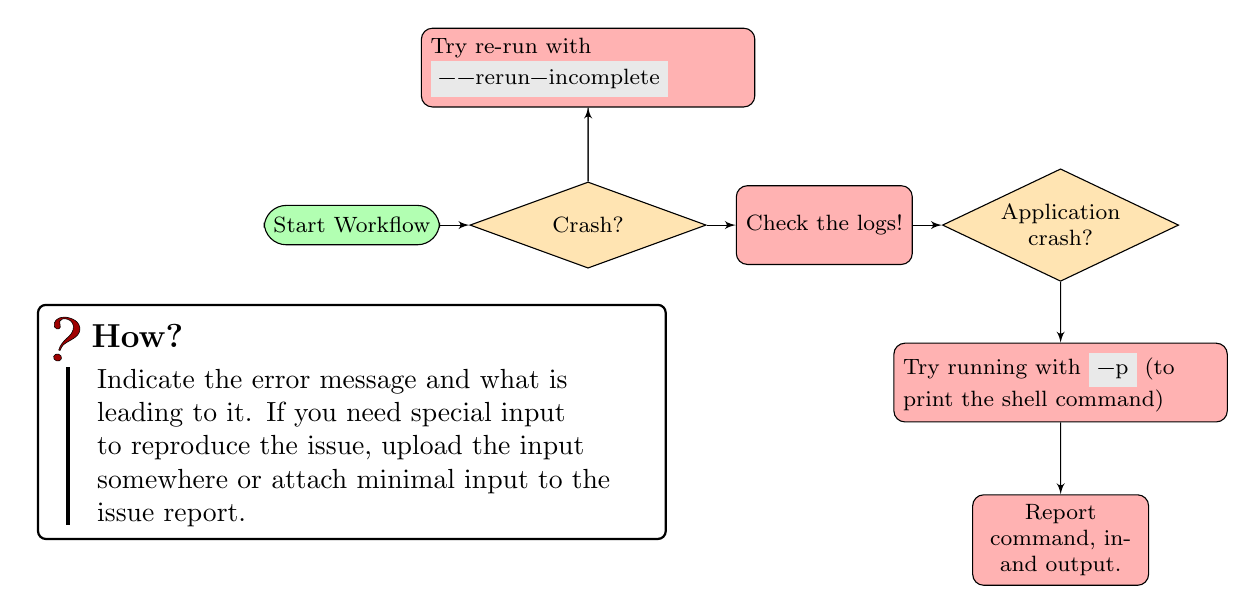
\begin{tikzpicture}[scale=0.8, auto, every node/.style={font=\footnotesize, >=stealth}]
			\tikzset{
				rblock/.style={draw, shape=rectangle,rounded corners=0.8em,align=center,minimum width=1.5cm,minimum height=0.5 cm, fill=green!30},
				decision/.style={diamond, 
					minimum width=3cm, 
					minimum height=1cm, 
					text centered, 
					draw=black, 
					fill=green!30},
				block/.style= {draw, rectangle,rounded corners, align=center,minimum width=2cm,minimum height=1cm,text width= 2cm, fill=red!30},
				block1/.style= {draw, rectangle,rounded corners, align=center,minimum width=3 cm,minimum height=1cm,text width= 3cm, fill=red!30},
				io/.style = {draw, shape=trapezium , trapezium left angle=60, trapezium right angle=120, minimum width=2 cm, text centered, draw=black, fill=blue!30},
				subblock/.style= {draw, rectangle,rounded corners, align=center,minimum width=1cm,minimum height=1cm, fill=red!30},
				superblock/.style= {draw, rectangle,rounded corners, align=center,minimum width=4 cm,minimum height=1cm, fill=red!30},
				decision/.style = {draw,diamond, aspect =2, minimum width=3cm, minimum height=1cm, text centered,text width= 1.8 cm, draw=black, inner sep=0pt, fill=orange!30},
				line/.style = {draw, -latex'}
			}
			\node [rblock]  (start) {Start Workflow};
			\node [decision, right of=start, xshift=2cm] (error) {Crash?};
			\node [block, above of=error, yshift=1cm,text width= 4cm] (rerun) {\begin{minipage}{4cm}
					Try re-run with \newline \altverb{--rerun-incomplete}
			\end{minipage}};
			\node [block, right of=error, xshift=2cm] (logs) {Check the logs!};
			\node [decision, right of=logs, xshift=2cm] (application) {Application crash?};
			
			\node [block, below of=application, text width=4cm, yshift=-1cm] (print)
			{\begin{minipage}{4cm}
					Try running with \altverb{-p} (to print the shell command)
			\end{minipage}};
			
			\node [block, below of=print, yshift=-1cm] (report) {Report command, in- and output.};
			
			\path [line] (start) -- (error);
			\path [line] (error) -- (rerun);
			\draw [line, -] (rerun) -- (error);
			\path [line] (error) -- (logs);
			
			\path [line] (logs) -- (application);
			
			\path [line] (application) -- (print);
			\path [line] (print) -- (report);
			
			\pause
			\node[below of=start, text width=8cm,font=\normalsize, yshift=-1.5cm] {\begin{question}[How?]
					Indicate the error message and what is leading to it. If you need special input to reproduce the issue, upload the input somewhere or attach minimal input to the issue report.
				\end{question}};
		   \onslide<1->	
		\end{tikzpicture}
	
	\end{adjustbox}
\end{frame}

%%%%%%%%%%%%%%%%%%%%%%%%%%%%%%%%%%%%%%%%%%%%%%%%%%%%%%%%%%%%%%%%%%%%%%%%%%%%%%%%
\begin{frame}
	\frametitle{Reporting Workflow Issues}
	\begin{question}[Where?]
		The issue tracker at your workflow. For \texttt{Snakemake} somewhere in the \lhref{https://snakemake.github.io/snakemake-workflow-catalog/}{catalog}. 
	\end{question}
	\pause
	\begin{question}[What?]
	   Check that it is you causing the error, e.\,g. undefined variables. \texttt{Snakemake} will inform you about the nature of the issue. Read the error output carefully. Report when sure it is not you.
	\end{question}
	\pause
	\begin{question}[How?]
		Indicate the error message and what is leading to it. If you need special input to reproduce the issue, upload the input somewhere or attach minimal input to the issue report.
	\end{question}
\end{frame}

%%%%%%%%%%%%%%%%%%%%%%%%%%%%%%%%%%%%%%%%%%%%%%%%%%%%%%%%%%%%%%%%%%%%%%%%%%%%%%%%
\begin{frame}
  \frametitle{Reporting \texttt{Snakemake} Issues}
  \begin{question}[Where to?]
  	 The \lhref{https://github.com/snakemake/snakemake/issues}{issue tracker of the \texttt{Snakemake} project}.
  \end{question}	
  \pause
  \begin{question}[What?]
  	Clearly unexpected behaviour. Or tracebacks pointing to \texttt{Snakemake} itself. 
  \end{question}
  \pause
  \begin{question}[How?]
  	Indicate the error message and what is leading to it (e.\,g. the command line you used). If you need special input to reproduce the issue, upload the input somewhere or attach minimal input to the issue report.
  \end{question}
\end{frame}

 % TODO: should include reporting issues
\end{document}

